\documentclass[a4paper,11pt]{article}

% \sloppy

%%%%%%%%%%%%%%%%%%%%%%%%%%%%%%%%%%%%%%%%%%%%%%%%%%%%%%%%%%%%
% PACKAGES
%%%%%%%%%%%%%%%%%%%%%%%%%%%%%%%%%%%%%%%%%%%%%%%%%%%%%%%%%%%%
\usepackage[utf8x]{inputenc}

\usepackage{amsmath, amssymb, url}

% \usepackage[pdftex]{graphicx,color}
\usepackage[pdftex,
		colorlinks=true,
		pagebackref=true,
		citecolor=darkgreen,
		linkcolor=darkblue,
		urlcolor=darkpurple,
	]{hyperref}

\hypersetup{
  pdftitle={IMITATOR User Manual},
  pdfauthor={\'Etienne Andr\'e}%
}


%%%%%%%%%%%%%%%%%%%%%%%%%%%%%%%%%%%%%%%%%%%%%%%%%%%%%%%%%%%%
% TIKZ
%%%%%%%%%%%%%%%%%%%%%%%%%%%%%%%%%%%%%%%%%%%%%%%%%%%%%%%%%%%%
\usepackage{pgf}
\usepackage{tikz}
\usetikzlibrary{arrows}
\usetikzlibrary{decorations.pathmorphing} 
% Couleurs

\definecolor{darkblue}{rgb}{0, 0, 0.7}
\definecolor{darkgreen}{rgb}{0, 0.5, 0}
\definecolor{darkpurple}{rgb}{0.7, 0, 0.7}


\definecolor{turquoise}{rgb}{0 0.41 0.41}
\definecolor{rouge}{rgb}{0.79 0.0 0.1}
\definecolor{vert}{rgb}{0.15 0.4 0.1}
\definecolor{mauve}{rgb}{0.6 0.4 0.8}
\definecolor{violet}{rgb}{0.58 0. 0.41}
\definecolor{orange}{rgb}{0.8 0.4 0.2}
\definecolor{bleu}{rgb}{0.39, 0.58, 0.93}
\definecolor{gris}{rgb}{0.6,0.6,0.6}
\definecolor{grisfonce}{rgb}{0.4,0.4,0.4}
% Jeu de couleurs pales
\definecolor{cpale1}{rgb}{1, 0.3, 0.3}
\definecolor{cpale2}{rgb}{0.3, 1, 0.3}
\definecolor{cpale3}{rgb}{0.3, 0.3, 1}
\definecolor{cpale4}{rgb}{1, 0.3, 1}
\definecolor{cpale5}{rgb}{1, 1, 0.3}
\definecolor{cpale6}{rgb}{0.3, 1, 1}
\definecolor{cpale7}{rgb}{0.9, 0.6, 0.2}
\definecolor{cpale8}{rgb}{0.7, 0.4, 1}
\definecolor{cpale9}{rgb}{0.5, 1, 0.75}
\definecolor{cpale10}{rgb}{0.8, 0.7, 0.6}
\definecolor{cpale11}{rgb}{0.6, 0.7, 0.8}
\definecolor{cpale12}{rgb}{0.2, 0.5, 0.9}
\definecolor{cpale13}{rgb}{0.5, 0.9, 0.2}
\definecolor{cpale14}{rgb}{0.9, 0.2, 0.5}
\definecolor{cpale15}{rgb}{0.7, 0.7, 0.7}
\definecolor{cpale16}{rgb}{0.8, 0.8, 0.5}

%%%%%%%%%%%%%%%%%%%%%%%%%%%%%%%%%%%%%%%%%%%%%%%%%%%%%%%%%%%%
% CONSTANTES
%%%%%%%%%%%%%%%%%%%%%%%%%%%%%%%%%%%%%%%%%%%%%%%%%%%%%%%%%%%%
%-%-%-%-%-%-%-%-%-%-%-%-%-%-%-%-%-%-%-%-%-%-%-%-%-%-%-%-%-%
% CONSTANTES MATHEMATIQUES
%-%-%-%-%-%-%-%-%-%-%-%-%-%-%-%-%-%-%-%-%-%-%-%-%-%-%-%-%-%
% Variables
\newcommand{\A}{\mathcal{A}}


% Ensembles
\newcommand{\grandn}{{\mathbb N}}
\newcommand{\grandq}{{\mathbb Q}}
\newcommand{\grandqplus}{{\mathbb Q}_{\geq 0}}
\newcommand{\grandr}{{\mathbb R}}
\newcommand{\grandrplus}{\grandr_{\geq 0}}
\newcommand{\grandz}{{\mathbb Z}}

% Unites
\newcommand{\micros}{\mathit{\mu s}}
\newcommand{\nanos}{ns}

% Noms
\newcommand{\tiling}{\mathit{Tiling}}
% \newcommand{\true}{\mathbf{true}}
\newcommand{\Ko}{K}
\newcommand{\pio}{\pi_0}
\newcommand{\piprime}{\pi}
\newcommand{\To}{T_0}
\newcommand{\Tprime}{T}

% Symboles
\newcommand{\emptystring}{$\epsilon$}
\newcommand{\fleche}[1]{\stackrel{#1}{\rightarrow}}
\newcommand{\Fleche}[1]{\stackrel{#1}{\Rightarrow}}
\newcommand{\steps}[0]{ {\rightarrow} }

% Booleens
\newcommand{\false}{{\tt false}}
\newcommand{\true}{{\tt true}}

% PARAMETRES RCP
\newcommand{\rcpFMax}{\mathit{rc\_fast\_max}}
\newcommand{\rcpFMin}{\mathit{rc\_fast\_min}}
\newcommand{\rcpSMax}{\mathit{rc\_slow\_max}}
\newcommand{\rcpSMin}{\mathit{rc\_slow\_min}}
\newcommand{\rcpD}{\mathit{delay}}

%-%-%-%-%-%-%-%-%-%-%-%-%-%-%-%-%-%-%-%-%-%-%-%-%-%-%-%-%-%
% ALGORITHMES
%-%-%-%-%-%-%-%-%-%-%-%-%-%-%-%-%-%-%-%-%-%-%-%-%-%-%-%-%-%
% Algorithmes PTA
\newcommand{\IM}{\mathit{IM}}
\newcommand{\carto}{\mathit{BC}}

%-%-%-%-%-%-%-%-%-%-%-%-%-%-%-%-%-%-%-%-%-%-%-%-%-%-%-%-%-%
% CONSTANTES DE CHAINES
%-%-%-%-%-%-%-%-%-%-%-%-%-%-%-%-%-%-%-%-%-%-%-%-%-%-%-%-%-%

% Outils
% \newcommand{\apron}{\textsc{Apron}}
\newcommand{\gdot}{\textsc{dot}}
\newcommand{\graphviz}{Graphviz}
\newcommand{\hytech}{{\sc HyTech}}
\newcommand{\imitator}{\textsc{Imitator}}
%%\newcommand{\imitatordeux}{\textsc{Imitator}\,II}
\newcommand{\imitatorExec}{\code{IMITATOR}}
% \newcommand{\imperator}{\textsc{ImpRator}}
\newcommand{\ocaml}{OCaml}
\newcommand{\phaver}{PHAVer}
% \newcommand{\polka}{NewPolka}
% \newcommand{\prism}{\textsc{Prism}}
\newcommand{\python}{Python}
% \newcommand{\red}{RED}
% \newcommand{\uppaal}{\textsc{Uppaal}}

% Current version
\newcommand{\imitatorversion}{2.5.0}



%%%%%%%%%%%%%%%%%%%%%%%%%%%%%%%%%%%%%%%%%%%%%%%%%%%%%%%%%%%%
% FORMATING
%%%%%%%%%%%%%%%%%%%%%%%%%%%%%%%%%%%%%%%%%%%%%%%%%%%%%%%%%%%%

\newcommand{\paragraphe}[1]{\paragraph{#1.}}

% Non terminal in a grammar
\newcommand{\nt}[1]{$\langle$\emph{#1}$\rangle$}
% Rule name in a grammar
\newcommand{\regleGrammaire}[1]{\bigskip \noindent \nt{#1} :: \\}
% Not taken into account in the grammar
\newcommand{\npec}[1]{\textcolor{green}{#1}}

\newcommand{\probleme}[2]{
	\medskip
	\noindent
	\fbox{
		\begin{minipage}{0.95\textwidth}
		\textbf{#1}
		
		#2
		\end{minipage}
	}
	
	\medskip
}

% \newcommand{\commentaire}[1]{\textcolor{red}{\textbf{$\Leftarrow$  #1 $\Rightarrow$}}} % commentaire dans un paragraphe
% \newcommand{\commentaire}[1]{}


% Code integre au texte
\newcommand{\code}[1]{\textbf{\texttt{#1}}}



%%%%%%%%%%%%%%%%%%%%%%%%%%%%%%%%%%%%%%%%%%%%%%%%%%%%%%%%%%%%
% IMITATOR FILES
%%%%%%%%%%%%%%%%%%%%%%%%%%%%%%%%%%%%%%%%%%%%%%%%%%%%%%%%%%%%
\usepackage{listings}
\newcommand{\FichierImitator}[1]{
  \lstset{language=Imitator}
  \lstinputlisting[columns=fixed, numbers=left, numberstyle=\tiny, breaklines=true, breakatwhitespace=true]{#1}
}

\lstdefinelanguage{Imitator}
  {morekeywords={
and, automaton, clock, discrete, do, end, endreach, False, forward, from, goto, if, in, init, initially, loc, locations, not, or, parameter, print, reach, region, sync, synclabs, True, var, wait, when, while
  },
  sensitive=false,
   morecomment=[l][\color{gray}]{--},
   morecomment=[s][keywordstyle]{"}{"},
 morecomment=[s]{/*}{*/},
 morecomment=[s]{(*}{*)},
}


%%%%%%%%%%%%%%%%%%%%%%%%%%%%%%%%%%%%%%%%%%%%%%%%%%%%%%%%%%%%
%%%%%%%%%%%%%%%%%%%%%%%%%%%%%%%%%%%%%%%%%%%%%%%%%%%%%%%%%%%%
%%%%%%%%%%%%%%%%%%%%%%%%%%%%%%%%%%%%%%%%%%%%%%%%%%%%%%%%%%%%

% Title Page
\title{IMITATOR User Manual\\{\Large Version \imitatorversion{}}}
\author{}
% \date{}

\begin{document}
\maketitle

\bigskip

\begin{center}
	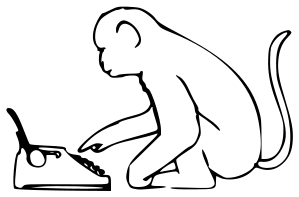
\includegraphics[width=0.40\textwidth]{include/monkey.png}
\end{center}

\bigskip


%%%%%%%%%%%%%%%%%%%%%%%%%%%%%%%%%%%%%%%%%%%%%%%%%%%%%%%%%%%%
%%%%%%%%%%%%%%%%%%%%%%%%%%%%%%%%%%%%%%%%%%%%%%%%%%%%%%%%%%%%
\begin{abstract}
\imitator{} is a tool for parameter synthesis in timed automata with stopwatches~\cite{AFKS12}.
It is based on the inverse method: given a reference valuation of the parameters, its generates a constraint such that the system behaves the same as under the reference valuation in terms of traces, i.e., alternating sequences of locations and actions.
% This is useful for safely relaxing some values of the reference valuation, and optimizing timing bounds of the system.
Besides the inverse method, \imitator{} also implements the ``behavioral cartography algorithm'', allowing to solve the following good parameters problem: find a set of valuations within a given rectangle for which the system behaves well.
% New features and optimizations of the tool are presented, and various examples of asynchronous circuits and communication protocols are studied.
We give here the installation requirements and the launching commands of \imitator{}, as well as the source code of a toy example.
\end{abstract}
%%%%%%%%%%%%%%%%%%%%%%%%%%%%%%%%%%%%%%%%%%%%%%%%%%%%%%%%%%%%
%%%%%%%%%%%%%%%%%%%%%%%%%%%%%%%%%%%%%%%%%%%%%%%%%%%%%%%%%%%%

\newpage
\tableofcontents
\newpage

% \pagestyle{fancyplain}
% \lhead{\fancyplain{}{\imitator{} \imitatorversion{} User Manual}}



%%%%%%%%%%%%%%%%%%%%%%%%%%%%%%%%%%%%%%%%%%%%%%%%%%%%%%%%%%%%
%%%%%%%%%%%%%%%%%%%%%%%%%%%%%%%%%%%%%%%%%%%%%%%%%%%%%%%%%%%%
\section{Introduction}
%%%%%%%%%%%%%%%%%%%%%%%%%%%%%%%%%%%%%%%%%%%%%%%%%%%%%%%%%%%%
%%%%%%%%%%%%%%%%%%%%%%%%%%%%%%%%%%%%%%%%%%%%%%%%%%%%%%%%%%%%


\imitator{} 2.5 (for \emph{Inverse Method for Inferring Time AbstracT behaviOR}) is a tool for parameter synthesis in the framework of real-time systems based on the inverse method~$\IM$ for Parametric Timed Automata (PTAs) augmented with stopwatches~\cite{AFKS12}.  % ,~\cite{ad94}
Different from CEGAR-based methods (see \cite{cgjlv00}), this algorithm for parameter synthesis makes use of a ``good'' parameter valuation~$\pio$ instead of a set of ``bad'' states~\cite{acef09}.
\imitator{} takes as input a network of PTAs with stopwatches
and a reference valuation~$\pio$; it synthesizes a constraint~$\Ko$ on the parameters such that (1) $\pio \models \Ko$ and (2) for all parameter valuation~$\piprime$ satisfying $\Ko$, the trace set (i.e., the discrete behavior) of~$\A$ under~$\piprime$ is the same as for~$\A$ under~$\pio$.
%This preserves in particular linear time properties, 
This provides the system with a criterion of \emph{robustness} (see, e.g., \cite{Markey11})
%, by formally guaranteeing a uniform discrete behavior 
around~$\pio$.

% It , that synchronize on shared actions
% The input syntax, inspired by~\hytech{}, allows the use of clocks (or stopwatches), rational-valued discrete variables, and parameters (i.e. unknown constants) to be used altogether in linear terms, within guards, invariants and updates.

% By iterating the inverse method on all integer points within a bounded reference parameter domain, we get a set of constraints %(``tiles'')
% such that, for every point in each such constraint, the time-abstract behavior is the same: this gives a behavioral cartography of the system~\cite{af10}.



%-%-%-%-%-%-%-%-%-%-%-%-%-%-%-%-%-%-%-%-%-%-%-%-%-%-%-%-%-%-%
\begin{figure}[ht!]
	% STYLES
	\tikzstyle{etiquette} = [draw=none, color=black]
	
% \tikzstyle{boite}=[text width=8em, text centered, minimum height=2.5em, rounded corners, very thick]
% \tikzstyle{input}=[boite, draw=green!20!gris, top color=green!50, bottom color=green!10!white]
% \tikzstyle{output}=[boite, draw=red!20!gris, top color=red!50, bottom color=red!5!white]
% \tikzstyle{imitator} = [boite, draw=blue!20!gris, text width=10em, minimum height=6em]

	
	\tikzstyle{boite}=[rectangle, draw=black, rounded corners, thick, draw=blue!40!black, top color=blue!5!white, bottom color=blue!20]
% 	\tikzstyle{imitator} = [boite]
% 	\tikzstyle{apron} = [boite, draw=yellow!20!gris, top color=yellow!70, bottom color=yellow!10!white]
% 	\tikzstyle{polka} = [apron]
% 	\tikzstyle{ppl} = [apron]
% 	\tikzstyle{dot} = [boite, draw=purple!20!gris, top color=purple!10!white, bottom color=purple!60]

	\tikzstyle{fleche} = [->, draw=black, semithick]
{

\centering

\begin{tikzpicture}[scale=0.72,  =>stealth']

	% Boites
	\draw[boite] (-5, 5.5) rectangle (-2, 6.5);
	\node [etiquette] at (-3.5, 6) {PTA};
	
	\draw[boite] (-5, 3.8) rectangle (-2, 5);
	\node [etiquette] at (-3.5, 4.4) {\begin{tabular}{c}Reference\\valuation $\pio$\end{tabular}};
	
	\draw[boite] (0, 4) rectangle (6, 6.5);
	\node [etiquette] at (3, 5.25) {\large \imitator{}};
	
% 	\draw[boite] (1, 4) rectangle (5, 5);
% 	\node [etiquette] at (3, 4.5) {PPL};
	
	\draw[boite] (8, 4.5) rectangle (12, 6);
	\node [etiquette] at (10, 5.25) {Constraint $\Ko$};
	
% 	\draw[boite] (8, 4) rectangle (12, 5);
% 	\node [etiquette] at (10, 4.5) {Trace set};

	% Fleches
	\path[fleche] (-2, 6) --++ (2, 0);
	\path[fleche] (-2, 4.4) --++ (2, 0);
% 	\path[fleche] (3.5, 4) --++ (0, -.5);
% 	\path[fleche] (2.5, 3.5) --++ (0, .5);
	\path[fleche] (6, 5.25) --++ (2, 0);
% 	\path[fleche] (6, 4.5) --++ (2, 0);

\end{tikzpicture}

}

\caption{Functional view of \imitator{}}
\label{fig:structure}
\end{figure}
%-%-%-%-%-%-%-%-%-%-%-%-%-%-%-%-%-%-%-%-%-%-%-%-%-%-%-%-%-%-%




%%%%%%%%%%%%%%%%%%%%%%%%%%%%%%%%%%%%%%%%%%%%%%%%%%%%%%%%%%%%%
%%%%%%%%%%%%%%%%%%%%%%%%%%%%%%%%%%%%%%%%%%%%%%%%%%%%%%%%%%%%%
\section{Installing IMITATOR}
%%%%%%%%%%%%%%%%%%%%%%%%%%%%%%%%%%%%%%%%%%%%%%%%%%%%%%%%%%%%%
%%%%%%%%%%%%%%%%%%%%%%%%%%%%%%%%%%%%%%%%%%%%%%%%%%%%%%%%%%%%%

Sources, binaries for Linux platforms, and installation instructions are available on \imitator{}'s Web page \cite{imitator_web}.


%%%%%%%%%%%%%%%%%%%%%%%%%%%%%%%%%%%%%%%%%%%%%%%%%%%%%%%%%%%%%
%%%%%%%%%%%%%%%%%%%%%%%%%%%%%%%%%%%%%%%%%%%%%%%%%%%%%%%%%%%%%
\section[Implementation]{General Structure and Implementation} \label{sec:implementation}
%%%%%%%%%%%%%%%%%%%%%%%%%%%%%%%%%%%%%%%%%%%%%%%%%%%%%%%%%%%%%
%%%%%%%%%%%%%%%%%%%%%%%%%%%%%%%%%%%%%%%%%%%%%%%%%%%%%%%%%%%%%



%%%%%%%%%%%%%%%%%%%%%%%%%%%%%%%%%%%%%%%%%%%%%%%%%%%%%%%%%%%%
\subsection{Inputs and Outputs}
%%%%%%%%%%%%%%%%%%%%%%%%%%%%%%%%%%%%%%%%%%%%%%%%%%%%%%%%%%%%

The input syntax of \imitator{} to describe the network of PTAs modeling the system is originally based on the \hytech{} syntax, with several improvements.
Actually, all standard \hytech{} files describing only PTAs (and not more general systems like linear hybrid automata\cite{achh92}) can be analyzed directly by \imitator{} with very minor changes.
% \footnote{An interface to accept as well files given using the \phaver{} syntax is currently being implemented.}.


%-%-%-%-%-%-%-%-%-%-%-%-%-%-%-%-%-%-%-%-%-%-%-%-%-%-%-%-%-%-%
\paragraphe{Inverse Method}
%-%-%-%-%-%-%-%-%-%-%-%-%-%-%-%-%-%-%-%-%-%-%-%-%-%-%-%-%-%-%
When calling \imitator{} to apply the inverse method algorithm, the tool takes as input two files, one describing the network of PTAs modeling the system, and the other describing the reference valuation.
As depicted in Figure~\ref{fig:ioIM}, it synthesizes a constraint on the parameters solving the inverse problem, as well as optionally the corresponding trace set under a graphical form.
The description of all the parametric reachable states can also be optionally output.

%-%-%-%-%-%-%-%-%-%-%-%-%-%-%-%-%-%-%-%-%-%-%-%-%-%-%-%-%-%-%
\begin{figure}[ht!]
\tikzstyle{input}=[draw, fill=green!40, text width=8em,
    text centered, minimum height=2.5em]
\tikzstyle{output}=[input, fill=red!40]
\tikzstyle{imitator} = [input, text width=10em, fill=blue!40,
    minimum height=6em, rounded corners]
\def\blockdist{2.3}
\def\edgedist{2.5}

{

\centering

\begin{tikzpicture}
    \node (imitator) [imitator] {\imitator{}};

    \path (imitator.162)+(-\blockdist,0) node (input1) [input] {PTA $\A$};
    \path (imitator.-162)+(-\blockdist,0) node (input2) [input] {Reference valuation $\pi_0$};
    \path (imitator.162)+(+3*\blockdist,0) node (output1) [output] {Constraint $K_0$ on the parameters};
    \path (imitator.-162)+(+3*\blockdist,0) node (output2) [output] {Trace set\\(graphical form)};

    \path [draw, ->] (input1) -- (imitator.west |- input1) ;
    \path [draw, ->] (input2) -- (imitator.west |- input2);
    \path [draw, ->] (imitator.east |- output1) -- (output1.west);
    \path [draw, ->] (imitator.east |- output2) -- (output2.west);
\end{tikzpicture}

}

\caption{\imitator{} inputs and outputs in inverse method mode}
\label{fig:ioIM}
\end{figure}
%-%-%-%-%-%-%-%-%-%-%-%-%-%-%-%-%-%-%-%-%-%-%-%-%-%-%-%-%-%-%


%-%-%-%-%-%-%-%-%-%-%-%-%-%-%-%-%-%-%-%-%-%-%-%-%-%-%-%-%-%-%
\paragraphe{Behavioral Cartography Algorithm}
%-%-%-%-%-%-%-%-%-%-%-%-%-%-%-%-%-%-%-%-%-%-%-%-%-%-%-%-%-%-%
When calling \imitator{} to apply the behavioral cartography algorithm, the tool takes as an input two files, one describing the network of PTAs modeling the system, and the other describing the reference rectangle, i.e., the bounds to consider for each parameter.
As depicted in Figure~\ref{fig:ioBC}, it synthesizes a list of tiles, as well as optionally the trace set corresponding to each tile under a graphical form.
The description of all the parametric reachable states for each tile may also optionally be output.

%-%-%-%-%-%-%-%-%-%-%-%-%-%-%-%-%-%-%-%-%-%-%-%-%-%-%-%-%-%-%
\begin{figure}[ht!]
\tikzstyle{input}=[draw, fill=green!40, text width=8em,
    text centered, minimum height=2.5em]
\tikzstyle{output}=[input, fill=red!40]
\tikzstyle{imitator} = [input, text width=10em, fill=blue!40,
    minimum height=6em, rounded corners]
\def\blockdist{2.3}
\def\edgedist{2.5}

{

\centering

\begin{tikzpicture}
    \node (imitator) [imitator] {\imitator{}};

    \path (imitator.162)+(-\blockdist,0) node (input1) [input] {PTA $\A$};
    \path (imitator.-162)+(-\blockdist,0) node (input2) [input] {Reference rectangle $V_0$};
    \path (imitator.162)+(+3*\blockdist,0) node (output1) [output] {List of tiles};
    \path (imitator.-162)+(+3*\blockdist,0) node (output2) [output] {List of trace sets\\(graphical form)};

    \path [draw, ->] (input1) -- (imitator.west |- input1) ;
    \path [draw, ->] (input2) -- (imitator.west |- input2);
    \path [draw, ->] (imitator.east |- output1) -- (output1.west);
    \path [draw, ->] (imitator.east |- output2) -- (output2.west);
\end{tikzpicture}

}

\caption{\imitator{} inputs and outputs in behavioral cartography mode}
\label{fig:ioBC}
\end{figure}
%-%-%-%-%-%-%-%-%-%-%-%-%-%-%-%-%-%-%-%-%-%-%-%-%-%-%-%-%-%-%

% 
% %-%-%-%-%-%-%-%-%-%-%-%-%-%-%-%-%-%-%-%-%-%-%-%-%-%-%-%-%-%-%
% \paragraphe{Internal Representation}
% %-%-%-%-%-%-%-%-%-%-%-%-%-%-%-%-%-%-%-%-%-%-%-%-%-%-%-%-%-%-%
% States are represented using a triple $(q, v, C)$ made of the current location~$q$ in each automaton, a value for each discrete variable\footnote{Discrete variables are syntactic sugar allowing to factorize several locations into a single one. In~\imitator{}, discrete variables are integer variables that can be updated using constants or other discrete variables.}~$v$, and a constraint $C$ on the clocks and the parameters.
% In order to optimize the test of equality between a new computed state and the set of states computed previously, the states are stored in a hash table as follows:
% to a given key $(q, v)$ of the hash table, we associate a list of constraints $C_1, \dots, C_n$, corresponding to the $n$ states $(q, v, C_1)$, \dots, $(q, v, C_n)$.
% % the location and the value for the discrete variables represent the key, and the value corresponds to 
% 
% Note that, unlike \hytech{}, \imitator{} uses exact arithmetics with unlimited precision.
% 
% Contrarily to \hytech{} which performs an \emph{a\,priori} static composition of the automata, thus leading to a dramatical explosion of the number of locations, \imitator{} performs an \emph{on-the-fly} composition of the automata.
% This \emph{on-the-fly} composition allows to analyze bigger systems, and decrease drastically the computation time compared to \imitator{}. % (see Section~\ref{sec:experiments}).

	


%%%%%%%%%%%%%%%%%%%%%%%%%%%%%%%%%%%%%%%%%%%%%%%%%%%%%%%%%%%%
\subsection{Features} \label{ss:features}
%%%%%%%%%%%%%%%%%%%%%%%%%%%%%%%%%%%%%%%%%%%%%%%%%%%%%%%%%%%%

\imitator{} (version \imitatorversion{}) includes the following features:

\begin{itemize}
	\item Analysis of a network of parametric timed automata augmented with stopwatches and discrete rational-valued variables;
	\item Reachability analysis: given a PTA~$\A$, compute the set of all the reachable states (as it is done in tools such as, e.g., \hytech{} and \phaver{});
	\item Inverse method algorithm: given a PTA~$\A$ and a reference valuation~$\pi_0$, synthesize a constraint guaranteeing the same trace set as for $\A[\pi_0]$;
	\item Behavioral cartography algorithm: given a PTA~$\A$ and a rectangular parameter domain~$V_0$, compute a list of tiles. Two different modes can be considered: (1) cover all the integer points of~$V_0$ or, (2) call a given number of times the inverse method on an integer point selected randomly within $V_0$ (which is interesting for rectangles containing a very big number of integer points but few different tiles);
	\item Automatic generation of the trace sets, for the reachability analysis and for both algorithms $\IM$ and $\carto$;
	\item Graphical output of the trace sets;
	\item Graphical output of the behavioral cartography;
	\item Optional use of the merging technique of \cite{AFS12}.
\end{itemize}


See Section~\ref{sss:options} for the list of options available when calling \imitator{}.





%%%%%%%%%%%%%%%%%%%%%%%%%%%%%%%%%%%%%%%%%%%%%%%%%%%%%%%%%%%%%
%%%%%%%%%%%%%%%%%%%%%%%%%%%%%%%%%%%%%%%%%%%%%%%%%%%%%%%%%%%%%
\section{How to Use \imitator{}} \label{sec:how}
%%%%%%%%%%%%%%%%%%%%%%%%%%%%%%%%%%%%%%%%%%%%%%%%%%%%%%%%%%%%%
%%%%%%%%%%%%%%%%%%%%%%%%%%%%%%%%%%%%%%%%%%%%%%%%%%%%%%%%%%%%%

%%%%%%%%%%%%%%%%%%%%%%%%%%%%%%%%%%%%%%%%%%%%%%%%%%%%%%%%%%%%%
\subsection{Installation}
%%%%%%%%%%%%%%%%%%%%%%%%%%%%%%%%%%%%%%%%%%%%%%%%%%%%%%%%%%%%%

See the installation files available on the website for the most up-to-date information.

In short, \imitator{} is written in \ocaml{}, and makes use of the following libraries:

\begin{itemize}
	\item The OCaml ExtLib library (Extended Standard Library for Objective Caml)
	\item The Parma Polyhedra Library (PPL)~\cite{bhz08}
        \item The GNU Multiple Precision Arithmetic Library (GMP)
\end{itemize}

Binaries and source code packages are available on \imitator{}'s Web page~\cite{imitator_web}.



%%%%%%%%%%%%%%%%%%%%%%%%%%%%%%%%%%%%%%%%%%%%%%%%%%%%%%%%%%%%%
\subsection{The \imitator{} Input File}
%%%%%%%%%%%%%%%%%%%%%%%%%%%%%%%%%%%%%%%%%%%%%%%%%%%%%%%%%%%%%

Examples of input files can be found on \imitator{}'s Web page~\cite{imitator_web}.
A complete example is given in Appendix~\ref{app:source}.
A tentative grammar is given in Appendix~\ref{app:grammar}.


%-%-%-%-%-%-%-%-%-%-%-%-%-%-%-%-%-%-%-%-%-%-%-%-%-%-%-%-%-%-%
\subsubsection{Variables}
%-%-%-%-%-%-%-%-%-%-%-%-%-%-%-%-%-%-%-%-%-%-%-%-%-%-%-%-%-%-%

% TO DO !
% \commentaire{Syntaxe des noms de variables}

Discrete variables, clocks and parameters variable names must be disjoint.

The synchronization label names may be identical to other names (automata or variables).
The automata names may be identical to other names (variables synchronization labels).

% TO DO !
% \commentaire{preciser labels synchronises tous ensemble}

% Any kind of variables (clocks, parameters, discrete, etc.) can be used.
% As in a standard \hytech{} file, they must be declared in the header of the file.

%-%-%-%-%-%-%-%-%-%-%-%-%-%-%-%-%-%-%-%-%-%-%-%-%-%-%-%-%-%-%
\subsubsection{Parametric Timed Automata}
%-%-%-%-%-%-%-%-%-%-%-%-%-%-%-%-%-%-%-%-%-%-%-%-%-%-%-%-%-%-%

See Appendix~\ref{app:grammar}.

%-%-%-%-%-%-%-%-%-%-%-%-%-%-%-%-%-%-%-%-%-%-%-%-%-%-%-%-%-%-%
\subsubsection{Initial region and $\pi_0$}
%-%-%-%-%-%-%-%-%-%-%-%-%-%-%-%-%-%-%-%-%-%-%-%-%-%-%-%-%-%-%

See Appendix~\ref{app:grammar}.


%%%%%%%%%%%%%%%%%%%%%%%%%%%%%%%%%%%%%%%%%%%%%%%%%%%%%%%%%%%%%
\subsection{Calling \imitator}
%%%%%%%%%%%%%%%%%%%%%%%%%%%%%%%%%%%%%%%%%%%%%%%%%%%%%%%%%%%%%

\imitator{} can be used with three different modes:

\begin{enumerate}
	\item Reachability analysis: given a PTA~$\A$, compute the whole set of reachable states from a given initial state.
	\item Inverse Method: given a PTA~$\A$ and a valuation~$\pi_0$ of the parameters, compute a constraint on the parameters guaranteeing the same behavior as under~$\pi_0$~\cite{acef09}.
	\item Behavioral Cartography Algorithm: given a PTA~$\A$ and a rectangle~$V_0$ (bounded interval of values for each parameter), compute a cartography of the system~\cite{af10}.
\end{enumerate}

We detail those three modes below.

% TO DO !
% \commentaire{preciser les sorties et endroits ou les fichiers sont g\'en\'er\'es)}


%-%-%-%-%-%-%-%-%-%-%-%-%-%-%-%-%-%-%-%-%-%-%-%-%-%-%-%-%-%-%
\subsubsection{Reachability Analysis} \label{ss:mode_reachability}
%-%-%-%-%-%-%-%-%-%-%-%-%-%-%-%-%-%-%-%-%-%-%-%-%-%-%-%-%-%-%

Given a PTA~$\A$, the reachability analysis computes the whole set of reachable states from a given initial state.
The syntax in this case is the following one:

\code{\imitatorExec{} <input\_file> -mode reachability [options]}

Note that there is no need to provide a $\pi_0$ or $V_0$ file in this case (if one is provided, it will be ignored).



%-%-%-%-%-%-%-%-%-%-%-%-%-%-%-%-%-%-%-%-%-%-%-%-%-%-%-%-%-%-%
\subsubsection{Inverse Method} \label{ss:mode_inversemethod}
%-%-%-%-%-%-%-%-%-%-%-%-%-%-%-%-%-%-%-%-%-%-%-%-%-%-%-%-%-%-%

Given a PTA~$\A$ and a valuation~$\pi_0$ of the parameters, the inverse method compute a constraint $K_0$ on the parameters guaranteeing that, for any $\pi \models K_0$, the trace sets of $\A[\pi]$ and $\A[\pi_0]$ are the same~\cite{acef09}.
The syntax in this case is the following one:

\code{\imitatorExec{} <input\_file> <pi0\_file> [-mode inversemethod] [options]}

Note that the \code{-mode inversemethod} option is not necessary, since the default value for \code{-mode} is precisely \code{inversemethod}.

Note that, unlike the algorithm given in~\cite{acef09}, at a given iteration, the $\pi_0$-incompatible state is selected deterministically, for efficiency reasons.
However, the $\pi_0$-incompatible inequality within a $\pi_0$-incompatible state is selected randomly, unless the \code{-no-random} option is activated.

In this case, \imitator{} outputs the resulting constraint $K_0$ on the standard output.
% Moreover, \imitator{} outputs the same two files as in the reachability analysis.


%-%-%-%-%-%-%-%-%-%-%-%-%-%-%-%-%-%-%-%-%-%-%-%-%-%-%-%-%-%-%
\subsubsection{Cartography} \label{ss:mode_cartography}
%-%-%-%-%-%-%-%-%-%-%-%-%-%-%-%-%-%-%-%-%-%-%-%-%-%-%-%-%-%-%

Given a PTA~$\A$ and a rectangle~$V_0$ (bounded interval of values for each parameter), the Behavioral Cartography Algorithm computes a cartography of the system~\cite{af10}.
Two possible variants of the algorithm can be used:
\begin{enumerate}
	\item The standard variant covers all the integer points within $V_0$.
	The syntax in this case is the following one:\\
	\code{\imitatorExec{} <input\_file> <V0\_file> [-mode cover] [options]}

	\item The alternative variant calls the inverse method a certain number of times on a random point $V_0$.
	The syntax in this case is the following one:\\
	\code{\imitatorExec{} <input\_file> <V0\_file> [-mode randomX] [options]}\\
	where \code{X} represents the number of random points to consider.
	If a point has already been generated before, the inverse method is not called.
	If a point belongs to one of the tiles computed before, the inverse method is not called neither.
	Therefore, in practice, the number of tiles generated is smaller than~\code{X}.
\end{enumerate}






%-%-%-%-%-%-%-%-%-%-%-%-%-%-%-%-%-%-%-%-%-%-%-%-%-%-%-%-%-%-%
\subsubsection{Options} \label{sss:options}
%-%-%-%-%-%-%-%-%-%-%-%-%-%-%-%-%-%-%-%-%-%-%-%-%-%-%-%-%-%-%

The options available for \imitator{} are explained in the following.

%------------------------------------------------------------
\paragraph{\code{-acyclic} (default: \code{false})}
%------------------------------------------------------------
Does not test if a new state was already encountered.
In a normal use, when \imitator{} encounters a new state, it checks if it has been encountered before.
This test may be time consuming for systems with a high number of reachable states.
For acyclic systems, all traces pass only once by a given location.
As a consquence, there are no cycles, so there should be no need to check if a given state has been encountered before.
This is the main purpose of this option.

However, be aware that, even for acyclic systems, several (different) traces can pass by the same state.
In such a case, if the \code{-acyclic} option is activated, \imitator{} will compute \emph{twice} the states after the state common to the two traces.
As a consequence, it is all but sure that activating this option will lead to an increase of speed.

Note also that activating this option for non-acyclic systems may lead to an infinite loop in \imitator{}.

%------------------------------------------------------------
\paragraph{\code{-cart} (default: \code{off})}
%------------------------------------------------------------

After execution of the behavioral cartography, plots the generated
zones as a \emph{PostScript} file. This option takes an integer which
limits the number of generated plots, where each plot represents the
projection of the parametric zones on two parameters. If the
considered rectangle $v_0$ is spanned by two parameters only, then
\code{-cart 1} will plot the projection of the generated zones on
these two parameters. 

This option makes use of the external utility \code{graph}, which is
part of the \emph{GNU plotting utils}, available on most Linux
platforms. The generated files will be located in the same directory
as the source files, unless option \code{-log-prefix} is used.

%------------------------------------------------------------
\paragraph{\code{-debug} (default: \code{standard})}
%------------------------------------------------------------

Give some debugging information, that may also be useful to have more details on the way \imitator{} works.
The admissible values for \code{-debug} are given below:

\begin{tabular}{@{} l @{\ \ } l}
 \code{nodebug} & Give only the resulting constraint \\
 \code{standard} & Give little information (number of steps, computation time)\\
 \code{low} & Give little additional debugging information\\
 \code{medium} & Give quite a lot of debugging information\\
 \code{high} & Give much debugging information\\
 \code{total} & Give really too much information\\
\end{tabular}


%------------------------------------------------------------
\paragraph{\code{-depth-limit <limit>} (default: \code{none})}
%------------------------------------------------------------
Limits the number of iterations in the $\mathit{Post}$ exploration, i.e., the depth of the traces.
In the cartography mode, this option gives a limit to \emph{each} call to the inverse method.

%------------------------------------------------------------
\paragraph{\code{-fancy} (default: \code{false})}
%------------------------------------------------------------

In the graphical output of the reachable states (see option \code{-with-dot}), 
provide detailed information on the local states of the composed automata.


%------------------------------------------------------------
\paragraph{\code{-inclusion} (default: \code{false})}
%------------------------------------------------------------
Consider an inclusion of region instead of the equality when performing the $\mathit{Post}$ operation.
In other terms, when encountering a new state, \imitator{} checks if the same state (same location and same constraint) has been encountered before and, if yes, does not consider this ``new'' state.
However, when the \code{-inclusion} option is activated, it suffices that a previous state with the same location and a constraint \emph{greater or equal} to the constraint of the new state has been encountered to stop the analysis.
This option corresponds to the way that, e.g., \hytech{} works, and suffices when one wants to check the \emph{non-reachability} of a given bad state.


%------------------------------------------------------------
\paragraph{\code{-log-prefix} (default: \code{<input\_file>})}
%------------------------------------------------------------
Set the prefix for log (\code{.states}) and graphical (\code{.gif}) files.


%------------------------------------------------------------
\paragraph{\code{-mode} (default: \code{inversemethod})}
%------------------------------------------------------------
The mode for \imitator{}.

\begin{tabular}{@{} l @{\ \ } l}
 \code{reachability} & Parametric reachability analysis  \\
 & (see Section~\ref{ss:mode_reachability}) \\
 \code{inversemethod} & Inverse method \\
 & (see Section~\ref{ss:mode_inversemethod}) \\
 \code{cover} & Behavioral Cartography Algorithm with full coverage \\
 & (see Section~\ref{ss:mode_cartography}) \\
 \code{randomXX} & Behavioral Cartography Algorithm with \code{XX} iterations \\
  & (see Section~\ref{ss:mode_cartography}) \\
\end{tabular}



%------------------------------------------------------------
\paragraph{\code{-no-random} (default: \code{false})}
%------------------------------------------------------------
No random selection of the $\pi_0$-incompatible inequality (select the first found).
By default, select an inequality in a random manner.


%------------------------------------------------------------
\paragraph{\code{-states-limit} (default: \code{none})}
%------------------------------------------------------------
Will try to stop after reaching this number of states.
Warning: the program may have to first finish computing the current iteration before stopping.


%------------------------------------------------------------
\paragraph{\code{-statistics} (default: \code{false})}
%------------------------------------------------------------
Print info on number of calls to PPL, and other statistics about memory and time.
Warning: enabling this option may slow down the analysis, and will certainly induce some extra computational time at the end.


%------------------------------------------------------------
\paragraph{\code{-step} (default: \code{1})}
%------------------------------------------------------------
Step for the behavioral cartography.


%------------------------------------------------------------
\paragraph{\code{-sync-auto-detect} (default: \code{false})}
%------------------------------------------------------------
\imitator{} considers that all the automata declaring a given synchronization label must be able to synchronize all together, so that the synchronization can happen.
By default, \imitator{} considers that the synchronization labels declared in an automaton are those declared in the \code{synclabs} section.
Therefore, if a synchronization label is declared but never used in (at least) one automaton, this label will never be synchronized in the execution\footnote{In such a case, the synchronization label is actually completely removed before the execution, in order to optimize the execution, and the user is warned of this removal.}.

The option \code{-sync-auto-detect} allows to detect automatically the synchronization labels in each automaton: the labels declared in the \code{synclabs} section are ignored, and the \imitator{} considers that only the labels really used in an automaton are those considered to be declared.


%------------------------------------------------------------
\paragraph{\code{-time-limit <limit>} (default: \code{none})}
%------------------------------------------------------------
Try to limit the execution time (the value \code{<limit>} is given in seconds).
Note that, in the current version of \imitator{}, the test of time limit is performed at the end of an iteration only (i.e., at the end of a given $\mathit{Post}$ iteration).
In the cartography mode, this option represents a \emph{global} time limit, not a limit for each call to the inverse method.


%------------------------------------------------------------
\paragraph{\code{-timed} (default: \code{false})}
%------------------------------------------------------------
Add a timing information to each output of the program.


%------------------------------------------------------------
\paragraph{\code{-with-dot} (default: \code{false})}
%------------------------------------------------------------
Graphical output using \gdot{}.
In this case, \imitator{} outputs a file \code{<input\_file>.jpg}, which is a graphical output in the jpg format, generated using \gdot{}, corresponding to the trace set.
% 	This graphical output is not generated in the case where the \code{-no-dot} option is activated.

Note that the location and the name of those two files can be changed using the \code{-log-prefix} option.



%------------------------------------------------------------
\paragraph{\code{-with-log} (default: \code{false})}
%------------------------------------------------------------
Generation of the files describing the reachable states.
In this case, \imitator{} outputs a file \code{<input\_file>.states} containing the set of all the reachable states, with their names and the associated constraint on the clocks and parameters.
If one wants to generate also the constraint on the parameters only, use the \code{-with-parametric-log} option.
This file also contains the source for the generation of the graphical file, using the \gdot{} syntax.


%------------------------------------------------------------
\paragraph{\code{-with-merging} (default: \code{false})}
%------------------------------------------------------------
Use the merging technique of \cite{AFS12}.


%------------------------------------------------------------
\paragraph{\code{-with-parametric-log } (default: \code{false})}
%------------------------------------------------------------
For any constraint on the clocks and the parameters in the description of the states in the log files,
add the constraint on the parameters only (i.e., eliminate clock variables).



%-%-%-%-%-%-%-%-%-%-%-%-%-%-%-%-%-%-%-%-%-%-%-%-%-%-%-%-%-%-%
\subsubsection{Examples of Calls}
%-%-%-%-%-%-%-%-%-%-%-%-%-%-%-%-%-%-%-%-%-%-%-%-%-%-%-%-%-%-%

%------------------------------------------------------------
\paragraph{\code{\imitatorExec{} flipflop.imi -mode reachability}}
%------------------------------------------------------------
Computes a reachability analysis on the automata described in file \code{flipflop.imi}.

%------------------------------------------------------------
\paragraph{\code{\imitatorExec{} flipflop.imi -mode reachability -with-dot -with-log}}
%------------------------------------------------------------
Computes a reachability analysis on the automata described in file \code{flipflop.imi}.
Will generate files \code{flipflop.imi.states}, containing the description of the reachable states, and \code{flipflop.imi.jpg} depicting the reachability graph.


%------------------------------------------------------------
\paragraph{\code{\imitatorExec{} flipflop.imi flipflop.pi0}}
%------------------------------------------------------------
Calls the inverse method on the automata described in file \code{flipflop.imi}, and the reference valuation $\pi_0$ given in file \code{flipflop.pi0}.
The resulting constraint $K_0$ will be given on the standard output.
% Moreover, \imitator{} will generate the file \code{flipflop.imi.states}, containing the description of the (parametric) states reachable under $K_0$, and the file \code{flipflop.imi.gif} depicting the reachability graph under any point $\pi \models K_0$.


% %------------------------------------------------------------
% \paragraph{\code{\imitatorExec{} flipflop.imi flipflop.pi0 -no-dot -no-log}}
% %------------------------------------------------------------
% Calls the inverse method on the automata described in file \code{flipflop.imi}, and the reference valuation given in file \code{flipflop.pi0}.
% The resulting constraint will be given on the standard output.
% No file will be generated.


%------------------------------------------------------------
\paragraph{\code{\imitatorExec{} flipflop.imi flipflop.pi0 -with-log -with-parametric-log}}
%------------------------------------------------------------
Calls the inverse method on the automata described in file \code{flipflop.imi}, and the reference valuation $\pi_0$ given in file \code{flipflop.pi0}.
The resulting constraint $K_0$ will be given on the standard output.
and \imitator{} will generate the file \code{flipflop.imi.states}, containing the description of the (parametric) states reachable under $K_0$.
Moveover, for any state in this file, both the constraint on the clocks and the parameters, and the constraint on the parameters will be given.
% \imitator{} will also generate the file \code{flipflop.imi.gif} depicting the reachability graph under any point $\pi \models K_0$.


%------------------------------------------------------------
\paragraph{\code{\imitatorExec{} SRlatch.imi SRlatch.v0 -mode cover}}
%------------------------------------------------------------
Calls the behavioral cartography algorithm on the automata described in file \code{flipflop.imi}, and the rectangle $V_0$ given in file \code{SRlatch.v0}.
The algorithm will cover (at least) all the integer points within $V_0$.
The resulting set of tiles will be given on the standard output.


%------------------------------------------------------------
\paragraph{\code{\imitatorExec{} SRlatch.imi SRlatch.v0 -mode cover -with-dot -with-log}}
%------------------------------------------------------------
Calls the behavioral cartography algorithm on the automata described in file \code{flipflop.imi}, and the rectangle $V_0$ given in file \code{SRlatch.v0}.
The algorithm will cover (at least) all the integer points within $V_0$.
The resulting set of tiles will be given on the standard output.
Given $n$ the number of generated tiles (i.e., the number of calls to the inverse method algorithm), the program will generate $n$ files of the form \code{SRlatch.imi\_$i$.states} (resp.~$n$ files of the form \code{SRlatch.imi\_$i$.jpg}) giving the description of the states (resp.~the reachability graph) of tile $i$, for $i = 1, \dots, n$.


%------------------------------------------------------------
\paragraph{\code{\imitatorExec{} SRlatch.imi SRlatch.v0 -mode random100 -with-dot}}
%------------------------------------------------------------
Calls the behavioral cartography algorithm on the automata described in file \code{flipflop.imi}, and the rectangle $V_0$ given in file \code{SRlatch.v0}.
The program will call the inverse method on 100 points randomly selected within $V_0$.
Since some points may be generated several times, or some points may belong to previously generated tiles (see Section~\ref{ss:mode_cartography}), the number $n$ of tiles generated will be such that $n \leq 100$.
The program will generate $n$ files of the form \code{SRlatch.imi\_$i$.jpg} giving the reachability graph of tile $i$, for $i = 1, \dots, n$.



%%%%%%%%%%%%%%%%%%%%%%%%%%%%%%%%%%%%%%%%%%%%%%%%%%%%%%%%%%%%%
%%%%%%%%%%%%%%%%%%%%%%%%%%%%%%%%%%%%%%%%%%%%%%%%%%%%%%%%%%%%%
\section{Example: SR-latch} \label{sec:example}
%%%%%%%%%%%%%%%%%%%%%%%%%%%%%%%%%%%%%%%%%%%%%%%%%%%%%%%%%%%%%
%%%%%%%%%%%%%%%%%%%%%%%%%%%%%%%%%%%%%%%%%%%%%%%%%%%%%%%%%%%%%



%-%-%-%-%-%-%-%-%-%-%-%-%-%-%-%-%-%-%-%-%-%-%-%-%-%-%-%-%-%-%
\begin{figure}
\centering
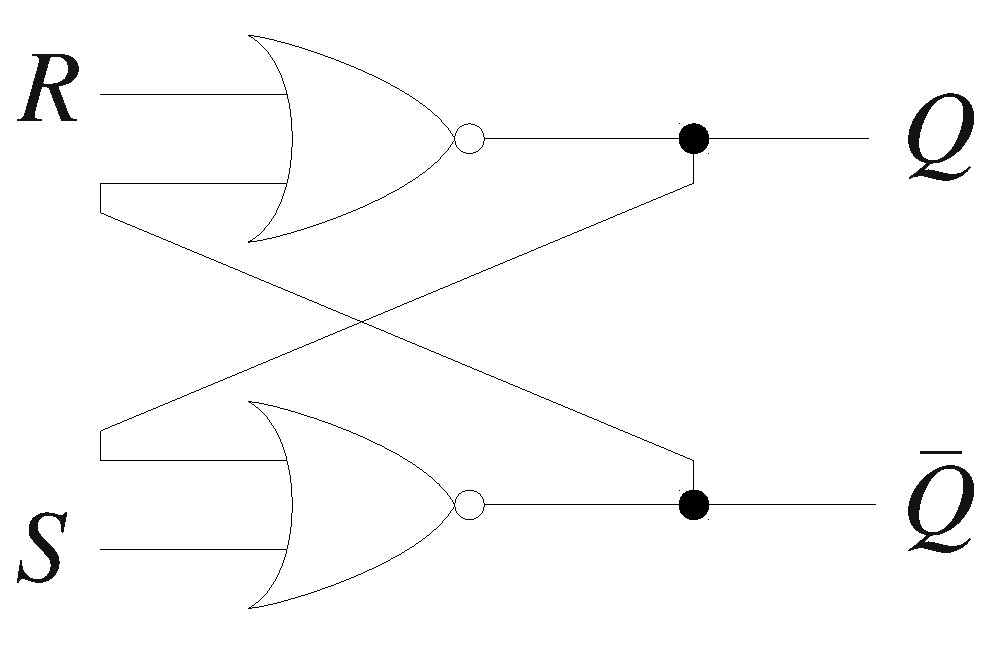
\includegraphics[width=0.30\textwidth]{include/SRlatch.pdf}
\ \ \ \ \ \ \ \ 
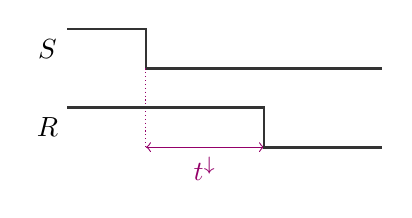
\begin{tikzpicture}[scale=.25]
	% STYLES
	\tikzstyle{signal} = [line width=1pt,draw=black!80]
	\tikzstyle{doublefleche} = [thin, <->, draw=violet]
	\tikzstyle{pointilles} = [thin, draw=violet, densely dotted]

	\tikzstyle{duree} = [below, pos=0.5, text=violet]

	% NOEUDS
	\node[] at (-1, 5) (S) {$S$};
	\node[] at (-1, 1) (R) {$R$};
	
	% S
	\path[signal]
		(0,6)
		-- ++ (4,0)
		-- ++ (0,-2) 
		-- ++ (12,0)
	;
	\path[doublefleche] (4, 0) -- ++(6, 0) node[duree] {$t^\downarrow$};
	\path[pointilles] (4, 4) -- ++(0, -4);

	% Q
	\path[signal]
		(0,2)
		-- ++ (10,0)
		-- ++ (0,-2) 
		-- ++ (6,0)
	;
\end{tikzpicture}

\caption{SR latch (left) and environment (right)}
\label{fig:srlatch}
\end{figure}
%-%-%-%-%-%-%-%-%-%-%-%-%-%-%-%-%-%-%-%-%-%-%-%-%-%-%-%-%-%-%

We consider a SR-latch described in, e.g., \cite{hh07}, and depicted on Fig.~\ref{fig:srlatch} left.
The possible configurations of the latch are the following ones:

\smallskip

{

\centering

\begin{tabular}{|c|c|c|c|}
	\hline
	$S$ & $R$ & $Q$ & $\overline{Q}$ \\
	\hline
	0 & 0 & latch & latch \\
	\hline
	0 & 1 & 0 & 1 \\
	\hline
	1 & 0 & 1 & 0 \\
	\hline
	1 & 1 & 0 & 0 \\
	\hline
\end{tabular}

}

\medskip

We consider an initial configuration with $R = S = 1$ and $Q = \overline{Q} = 0$.
As depicted in Fig.~\ref{fig:srlatch}, the signal~$S$ first goes down.
Then, the signal~$R$ goes down after a time~$t^\downarrow$.


We consider that the gate $\mathit{Nor}_1$ (resp. $\mathit{Nor}_2$) has a punctual parametric delay $\delta_1$ (resp. $\delta_2$).
Moreover, the parameter $t^\downarrow$ corresponds to the time duration between the fall of $S$ and the fall of $R$.


%%%%%%%%%%%%%%%%%%%%%%%%%%%%%%%%%%%%%%%%%%%%%%%%%%%%%%%%%%%%
\subsection{Parametric Reachability Analysis}
%%%%%%%%%%%%%%%%%%%%%%%%%%%%%%%%%%%%%%%%%%%%%%%%%%%%%%%%%%%%

We first perform a reachability analysis.
The launch command for \imitator{} is the following one:

\code{\imitatorExec{} SRlatch.imi -mode reachability}

Considering this environment, the trace set of this system is given in Fig.~\ref{fig:sr_parametric}, where the states $q_i$, $i = 0, \dots, 6$ correspond to the following values for each signal:

\smallskip

{

\centering

\begin{tabular}{|c||c|c|c|c|}
	\hline
	State & $S$ & $R$ & $Q$ & $\overline{Q}$ \\
	\hline
	$q_0$ & 1 & 1 & 0 & 0 \\
	\hline
	$q_1$ & 0 & 1 & 0 & 0 \\
	\hline
	$q_2$ & 0 & 0 & 0 & 0 \\
	\hline
	$q_3$ & 0 & 1 & 0 & 1 \\
	\hline
	$q_4$ & 0 & 0 & 0 & 1 \\
	\hline
	$q_5$ & 0 & 0 & 1 & 0 \\
	\hline
	$q_6$ & 0 & 0 & 0 & 1 \\
	\hline
\end{tabular}

}

\medskip

% %-%-%-%-%-%-%-%-%-%-%-%-%-%-%-%-%-%-%-%-%-%-%-%-%-%-%-%-%-%-%
% \begin{figure}
% \centering
% \footnotesize
% 
% \begin{tikzpicture}[scale=0.45, ->, >=stealth', auto, node distance=1.60cm, thin] % shorten >=1pt, 
%   \tikzstyle{state}=[circle, minimum size=15pt, draw=gris, text=black, inner sep=1.5pt]
% 
% 	\node[state, fill=cpale1] (Q0) at (0,3.5) {$q_0$};
% 	\node[state, fill=cpale2]         (Q1) at (4,2) {$q_1$};
% 	\node[state, fill=cpale3]         (Q2) at (4,5) {$q_2$};
% 	\node[state, fill=cpale4]         (Q3) at (8,0) {$q_3$};
% 	\node[state, fill=cpale5]         (Q4) at (8,2) {$q_4$};
% 	\node[state, fill=cpale5]         (Q5) at (8,5) {$q_5$};
% 	\node[state, fill=cpale6]         (Q6) at (8,8) {$q_6$};
% 	\node[state, fill=cpale7]         (Q7) at (12,2) {$q_7$};
% 	\node[state, fill=cpale7]         (Q8) at (12,0) {$q_8$};
% 	\node[state, fill=cpale8]         (Q9) at (12,4) {$q_9$};
% 	\node[state, fill=cpale7]        (Q10) at (12,6) {$q_{10}$};
% 	\node[state, fill=cpale8]        (Q11) at (12,8) {$q_{11}$};
% 
% 	\path
% 		(Q0) edge [double, below] node {$R^\downarrow$} (Q1)
% 		(Q0) edge [double] node {$S^\downarrow$} (Q2)
% 		(Q1) edge [double, below] node {$Q^\uparrow$} (Q3)
% 		(Q1) edge [double] node {$S^\downarrow$} (Q4)
% 		(Q2) edge [double, below] node {$R^\downarrow$} (Q5)
% 		(Q2) edge [double] node {$\overline{Q}^\uparrow$} (Q6)
% 		(Q3) edge [double] node {$S^\downarrow$} (Q8)
% 		(Q4) edge [double] node {$Q^\uparrow$} (Q7)
% 		(Q5) edge [double, below] node {$\overline{Q}^\uparrow$} (Q9)
% 		(Q5) edge [double] node {$Q^\uparrow$} (Q10)
% 		(Q6) edge [double] node {$R^\downarrow$} (Q11)
% 		;
% 
% \end{tikzpicture}
% \caption{Parametric reachability analysis of the SR latch}
% \label{fig:sr_parametric}
% \end{figure}
% %-%-%-%-%-%-%-%-%-%-%-%-%-%-%-%-%-%-%-%-%-%-%-%-%-%-%-%-%-%-%

%-%-%-%-%-%-%-%-%-%-%-%-%-%-%-%-%-%-%-%-%-%-%-%-%-%-%-%-%-%-%
\begin{figure}
\centering
\footnotesize

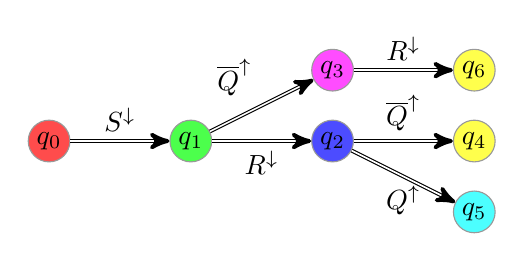
\begin{tikzpicture}[scale=0.45, ->, >=stealth', auto, node distance=1.60cm, thin] % shorten >=1pt, 
  \tikzstyle{state}=[circle, minimum size=15pt, draw=gris, text=black, inner sep=1.5pt]

	\node[state, fill=cpale1] (Q0) at (0,2) {$q_0$};
	\node[state, fill=cpale2]         (Q1) at (4,2) {$q_1$};
	\node[state, fill=cpale3]         (Q2) at (8,2) {$q_2$};
	\node[state, fill=cpale4]         (Q3) at (8,4) {$q_3$};
	\node[state, fill=cpale5]         (Q4) at (12,2) {$q_4$};
	\node[state, fill=cpale6]         (Q5) at (12,0) {$q_5$};
	\node[state, fill=cpale5]         (Q6) at (12,4) {$q_6$};

	\path
		(Q0) edge [double] node {$S^\downarrow$} (Q1)
		(Q1) edge [double, below] node {$R^\downarrow$} (Q2)
		(Q1) edge [double] node {$\overline{Q}^\uparrow$} (Q3)
		(Q2) edge [double] node {$\overline{Q}^\uparrow$} (Q4)
		(Q2) edge [double, below] node {$Q^\uparrow$} (Q5)
		(Q3) edge [double] node {$R^\downarrow$} (Q6)
		;

\end{tikzpicture}
\caption{Parametric reachability analysis of the SR latch}
\label{fig:sr_parametric}
\end{figure}
%-%-%-%-%-%-%-%-%-%-%-%-%-%-%-%-%-%-%-%-%-%-%-%-%-%-%-%-%-%-%

% 
% %%%%%%%%%%%%%%%%%%%%%%%%%%%%%%%%%%%%%%%%%%%%%%%%%%%%%%%%%%%%
% \subsection{Inverse Method}
% %%%%%%%%%%%%%%%%%%%%%%%%%%%%%%%%%%%%%%%%%%%%%%%%%%%%%%%%%%%%
% 
% We consider the following reference valuation $\pi_0$ of the parameters:
% 
% {\centering
% 
% \small
% 
% \begin{tabular}{r @{\ =\ } l @{\ \ \ \ \ \ } r @{\ =\ } l @{\ \ \ \ \ \ } r @{\ =\ } l @{\ \ \ \ \ \ } r @{\ =\ } l}
% $\delta_1^-$ & $1$  & $\delta_1^+$ & $4$ & $\delta_2^-$ & $2$ & $\delta_2^+$ & $5$ \\
% $T_R$ & $11$ & $T_S$ & $10$ \\
% \end{tabular}
% 
% }
% 
% Considering this environment and this reference valuation, the trace set is given in Fig.~\commentaire{to do}.
% 
% The constraint $K_0$ output by \imitator{} is the following one:
% 
% \smallskip
% 
% {\centering
% 
% %  t_S_down + dNor2_u >= t_R_down + dNor1_l
% %  & dNor1_u >= dNor1_l
% %  & dNor2_u >= dNor2_l
% %  & t_S_down >= 0
% %  & t_R_down > t_S_down
% %  & t_S_down + dNor2_l > t_R_down
% %  & t_R_down + dNor1_u >= t_S_down + dNor2_l
% %  & dNor1_l >= 0
% 
% \small
% \begin{tabular}{r r @{\ } c @{\ } l @{\ \ \ \ \ } r r @{\ } c @{\ } l}
% & $T_S + \delta_2^+ $ & $ \geq $ & $ t_R + \delta_1^- $ &
% $\land$ & $T_S$ & $ \geq $ & $ 0 $ \\
% $\land$ & $T_S + \delta_2^- $ & $>$ & $T_R$ &
% $\land$ & $T_R $ & $>$ & $ T_S $ \\
% $\land$ & $T_R + \delta_1^+ $ & $ \geq $ & $ T_S + \delta_2^- $ &
% $\land$ & $\delta_1^- $ & $ \geq $ & $ 0 $\\
% \end{tabular}
% 
% }
% 
% \medskip
% 
% We checked that the trace sets under the $\pi_0$ and $K_0$ are the same.
% 

%%%%%%%%%%%%%%%%%%%%%%%%%%%%%%%%%%%%%%%%%%%%%%%%%%%%%%%%%%%%
\subsection{Behavioral Cartography Algorithm}
%%%%%%%%%%%%%%%%%%%%%%%%%%%%%%%%%%%%%%%%%%%%%%%%%%%%%%%%%%%%


Using \imitator{}, we now perform a behavioral cartography of this system.
We consider the following rectangle $V_0$ for the parameters:

\smallskip

{\centering

% \small

\begin{tabular}{r @{\ $\in$ \ } l}
$ t^\downarrow $ & $[0, 10]$ \\
$ \delta_1 $ & $[0, 10]$ \\
$ \delta_2 $ & $[0, 10]$ \\
\end{tabular}

}

\smallskip

The launch command for \imitator{} is the following one:

\code{\imitatorExec{} SRlatch.imi SRlatch.v0 -mode cover}

We get the following six behavioral tiles.
Note that the graphical outputs, automatically generated in the \code{jpg} format by~\imitator{} using the \code{-with-dot} option, were rewritten in \LaTeX{} in this document.


%-%-%-%-%-%-%-%-%-%-%-%-%-%-%-%-%-%-%-%-%-%-%-%-%-%-%-%-%-%-%
\paragraph*{Tile 1.}
%-%-%-%-%-%-%-%-%-%-%-%-%-%-%-%-%-%-%-%-%-%-%-%-%-%-%-%-%-%-%
This tile corresponds to the values of the parameters verifying the following constraint:

$$ t^\downarrow = \delta_2
\ \ \land \ \ 
 \delta_1 = 0 $$

The trace set of this tile is given in Fig.~\ref{fig:sr_tile_1}.

%-%-%-%-%-%-%-%-%-%-%-%-%-%-%-%-%-%-%-%-%-%-%-%-%-%-%-%-%-%-%
\begin{figure}[ht]
\centering
\footnotesize

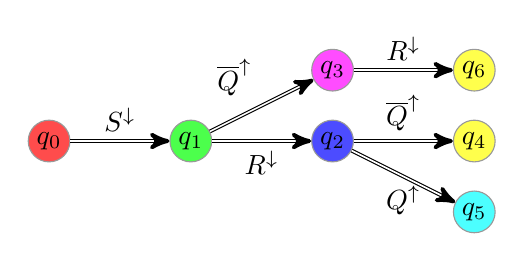
\begin{tikzpicture}[scale=0.45, ->, >=stealth', auto, node distance=1.60cm, thin] % shorten >=1pt, 
  \tikzstyle{state}=[circle, minimum size=15pt, draw=gris, text=black, inner sep=1.5pt]

	\node[state, fill=cpale1] (Q0) at (0,2) {$q_0$};
	\node[state, fill=cpale2]         (Q1) at (4,2) {$q_1$};
	\node[state, fill=cpale3]         (Q2) at (8,2) {$q_2$};
	\node[state, fill=cpale4]         (Q3) at (8,4) {$q_3$};
	\node[state, fill=cpale5]         (Q4) at (12,2) {$q_4$};
	\node[state, fill=cpale6]         (Q5) at (12,0) {$q_5$};
	\node[state, fill=cpale5]         (Q6) at (12,4) {$q_6$};

	\path
		(Q0) edge [double] node {$S^\downarrow$} (Q1)
		(Q1) edge [double, below] node {$R^\downarrow$} (Q2)
		(Q1) edge [double] node {$\overline{Q}^\uparrow$} (Q3)
		(Q2) edge [double] node {$\overline{Q}^\uparrow$} (Q4)
		(Q2) edge [double, below] node {$Q^\uparrow$} (Q5)
		(Q3) edge [double] node {$R^\downarrow$} (Q6)
		;

\end{tikzpicture}
\caption{Trace set of tile 1 for the SR latch}
\label{fig:sr_tile_1}
\end{figure}
%-%-%-%-%-%-%-%-%-%-%-%-%-%-%-%-%-%-%-%-%-%-%-%-%-%-%-%-%-%-%

Since $t^\downarrow = \delta_2$, $R^\downarrow$ and $\overline{Q}^\uparrow$ will occur at the same time.
Thus, the order of those two events is unspecified, which explains the choice between going to $q_2$ or $q_3$.
When in state $q_2$, either $Q^\uparrow$ can occur (since $\delta_1 = 0$), in which case the system is stable, or $\overline{Q}^\uparrow$ can occur, which also leads to stability.


%-%-%-%-%-%-%-%-%-%-%-%-%-%-%-%-%-%-%-%-%-%-%-%-%-%-%-%-%-%-%
\paragraph*{Tile 2.}
%-%-%-%-%-%-%-%-%-%-%-%-%-%-%-%-%-%-%-%-%-%-%-%-%-%-%-%-%-%-%
This tile corresponds to the values of the parameters verifying the following constraint:

$$ t^\downarrow = \delta_2
\ \ \land \ \ 
\delta_1 > 0 $$

The trace set of this tile is given in Fig.~\ref{fig:sr_tile_2}.

%-%-%-%-%-%-%-%-%-%-%-%-%-%-%-%-%-%-%-%-%-%-%-%-%-%-%-%-%-%-%
\begin{figure}[ht]
\centering
\footnotesize

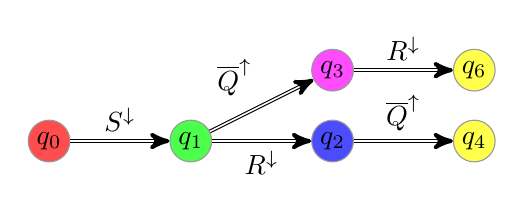
\begin{tikzpicture}[scale=0.45, ->, >=stealth', auto, node distance=1.60cm, thin] % shorten >=1pt, 
  \tikzstyle{state}=[circle, minimum size=15pt, draw=gris, text=black, inner sep=1.5pt]

	\node[state, fill=cpale1] (Q0) at (0,2) {$q_0$};
	\node[state, fill=cpale2]         (Q1) at (4,2) {$q_1$};
	\node[state, fill=cpale3]         (Q2) at (8,2) {$q_2$};
	\node[state, fill=cpale4]         (Q3) at (8,4) {$q_3$};
	\node[state, fill=cpale5]         (Q4) at (12,2) {$q_4$};
% 	\node[state, fill=cpale6]         (Q5) at (12,0) {$q_5$};
	\node[state, fill=cpale5]         (Q6) at (12,4) {$q_6$};

	\path
		(Q0) edge [double] node {$S^\downarrow$} (Q1)
		(Q1) edge [double, below] node {$R^\downarrow$} (Q2)
		(Q1) edge [double] node {$\overline{Q}^\uparrow$} (Q3)
		(Q2) edge [double] node {$\overline{Q}^\uparrow$} (Q4)
% 		(Q2) edge [double, below] node {$Q^\uparrow$} (Q5)
		(Q3) edge [double] node {$R^\downarrow$} (Q6)
		;

\end{tikzpicture}
\caption{Trace set of tile 2 for the SR latch}
\label{fig:sr_tile_2}
\end{figure}
%-%-%-%-%-%-%-%-%-%-%-%-%-%-%-%-%-%-%-%-%-%-%-%-%-%-%-%-%-%-%

Since $t^\downarrow = \delta_2$, $R^\downarrow$ and $\overline{Q}^\uparrow$ will occur at the same time.
Thus, the order of those two events is unspecified, which explains the choice between going to $q_2$ or $q_3$.
When in state $q_2$, $Q^\uparrow$ can not occur (since $\delta_1 > 0$), so $\overline{Q}^\uparrow$ occurs immediately after $R^\downarrow$, which leads to stability.


%-%-%-%-%-%-%-%-%-%-%-%-%-%-%-%-%-%-%-%-%-%-%-%-%-%-%-%-%-%-%
\paragraph*{Tile 3.}
%-%-%-%-%-%-%-%-%-%-%-%-%-%-%-%-%-%-%-%-%-%-%-%-%-%-%-%-%-%-%
This tile corresponds to the values of the parameters verifying the following constraint:

$$ \delta_2 > t^\downarrow + \delta_1 $$

The trace set of this tile is given in Fig.~\ref{fig:sr_tile_3}.

%-%-%-%-%-%-%-%-%-%-%-%-%-%-%-%-%-%-%-%-%-%-%-%-%-%-%-%-%-%-%
\begin{figure}[ht]
\centering
\footnotesize

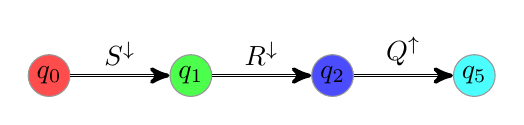
\begin{tikzpicture}[scale=0.45, ->, >=stealth', auto, node distance=1.60cm, thin] % shorten >=1pt, 
  \tikzstyle{state}=[circle, minimum size=15pt, draw=gris, text=black, inner sep=1.5pt]

	\node[state, fill=cpale1] (Q0) at (0,2) {$q_0$};
	\node[state, fill=cpale2]         (Q1) at (4,2) {$q_1$};
	\node[state, fill=cpale3]         (Q2) at (8,2) {$q_2$};
% 	\node[state, fill=cpale4]         (Q3) at (8,4) {$q_3$};
% 	\node[state, fill=cpale5]         (Q4) at (12,2) {$q_4$};
	\node[state, fill=cpale6]         (Q5) at (12,2) {$q_5$};
% 	\node[state, fill=cpale5]         (Q6) at (12,4) {$q_6$};

	\path
		(Q0) edge [double] node {$S^\downarrow$} (Q1)
		(Q1) edge [double] node {$R^\downarrow$} (Q2)
% 		(Q1) edge [double] node {$\overline{Q}^\uparrow$} (Q3)
% 		(Q2) edge [double] node {$\overline{Q}^\uparrow$} (Q4)
		(Q2) edge [double] node {$Q^\uparrow$} (Q5)
% 		(Q3) edge [double] node {$R^\downarrow$} (Q6)
		;

\end{tikzpicture}
\caption{Trace set of tile 3 for the SR latch}
\label{fig:sr_tile_3}
\end{figure}
%-%-%-%-%-%-%-%-%-%-%-%-%-%-%-%-%-%-%-%-%-%-%-%-%-%-%-%-%-%-%

In this case, since $\delta_2 > t^\downarrow + \delta_1 $, $S^\downarrow$ will occur before the gate $\mathit{Nor}_2$ has the time to change.
For the same reason, $Q^\uparrow$ will change before $\mathit{Nor}_1$ has the time to change.
With $Q = 1$, the system is now stable: $\mathit{Nor}_1$ does not change.


%-%-%-%-%-%-%-%-%-%-%-%-%-%-%-%-%-%-%-%-%-%-%-%-%-%-%-%-%-%-%
\paragraph*{Tile 4.}
%-%-%-%-%-%-%-%-%-%-%-%-%-%-%-%-%-%-%-%-%-%-%-%-%-%-%-%-%-%-%
This tile corresponds to the values of the parameters verifying the following constraint:

% t_down + dNor1 = dNor2                                                                   
%  & dNor2 >= dNor1                                                                           
%  & dNor1 > 0  

$$ t^\downarrow + \delta_1 = \delta_2 \ \ \land \ \ \delta_2 \geq \delta_1 \ \ \land \ \ \delta_1 > 0$$

The trace set of this tile is given in Fig.~\ref{fig:sr_tile_4}.

%-%-%-%-%-%-%-%-%-%-%-%-%-%-%-%-%-%-%-%-%-%-%-%-%-%-%-%-%-%-%
\begin{figure}[ht]
\centering
\footnotesize

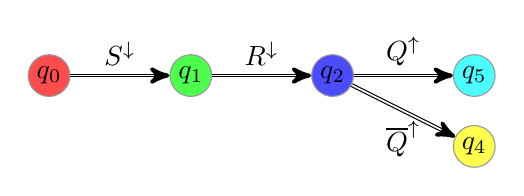
\begin{tikzpicture}[scale=0.45, ->, >=stealth', auto, node distance=1.60cm, thin] % shorten >=1pt, 
  \tikzstyle{state}=[circle, minimum size=15pt, draw=gris, text=black, inner sep=1.5pt]

	\node[state, fill=cpale1] (Q0) at (0,2) {$q_0$};
	\node[state, fill=cpale2]         (Q1) at (4,2) {$q_1$};
	\node[state, fill=cpale3]         (Q2) at (8,2) {$q_2$};
% 	\node[state, fill=cpale4]         (Q3) at (8,4) {$q_3$};
	\node[state, fill=cpale5]         (Q4) at (12,0) {$q_4$};
	\node[state, fill=cpale6]         (Q5) at (12,2) {$q_5$};
% 	\node[state, fill=cpale5]         (Q6) at (12,4) {$q_6$};

	\path
		(Q0) edge [double] node {$S^\downarrow$} (Q1)
		(Q1) edge [double] node {$R^\downarrow$} (Q2)
% 		(Q1) edge [double] node {$\overline{Q}^\uparrow$} (Q3)
		(Q2) edge [double, below] node {$\overline{Q}^\uparrow$} (Q4)
		(Q2) edge [double] node {$Q^\uparrow$} (Q5)
% 		(Q3) edge [double] node {$R^\downarrow$} (Q6)
		;

\end{tikzpicture}
\caption{Trace set of tile 4 for the SR latch}
\label{fig:sr_tile_4}
\end{figure}
%-%-%-%-%-%-%-%-%-%-%-%-%-%-%-%-%-%-%-%-%-%-%-%-%-%-%-%-%-%-%

Since $t^\downarrow + \delta_1 = \delta_2$, both $Q^\uparrow$ or $\overline{Q}^\uparrow$ can occur.
Once one of them occured, the system gets stable, and no other change occurs.



%-%-%-%-%-%-%-%-%-%-%-%-%-%-%-%-%-%-%-%-%-%-%-%-%-%-%-%-%-%-%
\paragraph*{Tile 5.}
%-%-%-%-%-%-%-%-%-%-%-%-%-%-%-%-%-%-%-%-%-%-%-%-%-%-%-%-%-%-%
This tile corresponds to the values of the parameters verifying the following constraint:

% dNor2 > t_down
%  & t_down + dNor1 > dNor2
 
$$ \delta_2 > t^\downarrow
\ \ \land \ \ 
 t^\downarrow + \delta_1 > \delta_2 $$

The trace set of this tile is given in Fig.~\ref{fig:sr_tile_5}.

%-%-%-%-%-%-%-%-%-%-%-%-%-%-%-%-%-%-%-%-%-%-%-%-%-%-%-%-%-%-%
\begin{figure}[ht]
\centering
\footnotesize

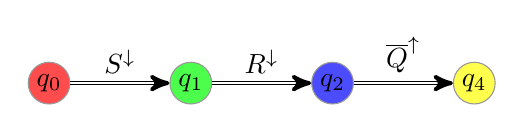
\begin{tikzpicture}[scale=0.45, ->, >=stealth', auto, node distance=1.60cm, thin] % shorten >=1pt, 
  \tikzstyle{state}=[circle, minimum size=15pt, draw=gris, text=black, inner sep=1.5pt]

	\node[state, fill=cpale1] (Q0) at (0,2) {$q_0$};
	\node[state, fill=cpale2]         (Q1) at (4,2) {$q_1$};
	\node[state, fill=cpale3]         (Q2) at (8,2) {$q_2$};
% 	\node[state, fill=cpale4]         (Q3) at (8,4) {$q_3$};
	\node[state, fill=cpale5]         (Q4) at (12,2) {$q_4$};
% 	\node[state, fill=cpale6]         (Q5) at (12,0) {$q_5$};
% 	\node[state, fill=cpale5]         (Q6) at (12,4) {$q_6$};

	\path
		(Q0) edge [double] node {$S^\downarrow$} (Q1)
		(Q1) edge [double] node {$R^\downarrow$} (Q2)
% 		(Q1) edge [double] node {$\overline{Q}^\uparrow$} (Q3)
		(Q2) edge [double] node {$\overline{Q}^\uparrow$} (Q4)
% 		(Q2) edge [double, below] node {$Q^\uparrow$} (Q5)
% 		(Q3) edge [double] node {$R^\downarrow$} (Q6)
		;

\end{tikzpicture}
\caption{Trace set of tile 5 for the SR latch}
\label{fig:sr_tile_5}
\end{figure}
%-%-%-%-%-%-%-%-%-%-%-%-%-%-%-%-%-%-%-%-%-%-%-%-%-%-%-%-%-%-%

Since $\delta_2 > t^\downarrow$, the gate $\mathit{Nor}_2$ can not change before $R^\downarrow$ occurs.
However, since $t^\downarrow + \delta_1 > \delta_2$, the gate $\mathit{Nor}_2$ changes before $Q^\uparrow$ can occur, thus leading to event~$\overline{Q}^\uparrow$.


%-%-%-%-%-%-%-%-%-%-%-%-%-%-%-%-%-%-%-%-%-%-%-%-%-%-%-%-%-%-%
\paragraph*{Tile 6.}
%-%-%-%-%-%-%-%-%-%-%-%-%-%-%-%-%-%-%-%-%-%-%-%-%-%-%-%-%-%-%
This tile corresponds to the values of the parameters verifying the following constraint:

% t_down > dNor2
%  & dNor2 >= 0
%  & dNor1 >= 0
 
$$ t^\downarrow > \delta_2$$

The trace set of this tile is given in Fig.~\ref{fig:sr_tile_6}.

%-%-%-%-%-%-%-%-%-%-%-%-%-%-%-%-%-%-%-%-%-%-%-%-%-%-%-%-%-%-%
\begin{figure}[ht]
\centering
\footnotesize

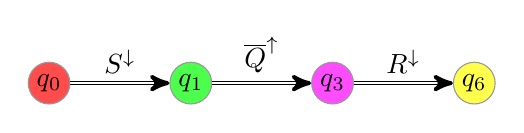
\begin{tikzpicture}[scale=0.45, ->, >=stealth', auto, node distance=1.60cm, thin] % shorten >=1pt, 
  \tikzstyle{state}=[circle, minimum size=15pt, draw=gris, text=black, inner sep=1.5pt]

	\node[state, fill=cpale1] (Q0) at (0,2) {$q_0$};
	\node[state, fill=cpale2]         (Q1) at (4,2) {$q_1$};
% 	\node[state, fill=cpale3]         (Q2) at (8,2) {$q_2$};
	\node[state, fill=cpale4]         (Q3) at (8,2) {$q_3$};
% 	\node[state, fill=cpale5]         (Q4) at (12,2) {$q_4$};
% 	\node[state, fill=cpale6]         (Q5) at (12,0) {$q_5$};
	\node[state, fill=cpale5]         (Q6) at (12,2) {$q_6$};

	\path
		(Q0) edge [double] node {$S^\downarrow$} (Q1)
% 		(Q1) edge [double, below] node {$R^\downarrow$} (Q2)
		(Q1) edge [double] node {$\overline{Q}^\uparrow$} (Q3)
% 		(Q2) edge [double] node {$\overline{Q}^\uparrow$} (Q4)
% 		(Q2) edge [double, below] node {$Q^\uparrow$} (Q5)
		(Q3) edge [double] node {$R^\downarrow$} (Q6)
		;

\end{tikzpicture}
\caption{Trace set of tile 6 for the SR latch}
\label{fig:sr_tile_6}
\end{figure}
%-%-%-%-%-%-%-%-%-%-%-%-%-%-%-%-%-%-%-%-%-%-%-%-%-%-%-%-%-%-%

Since $t^\downarrow > \delta_2$, $\overline{Q}^\uparrow$ occurs before $S^\downarrow$.
The system is then stable.


%-%-%-%-%-%-%-%-%-%-%-%-%-%-%-%-%-%-%-%-%-%-%-%-%-%-%-%-%-%-%
\paragraph*{Cartography.}
%-%-%-%-%-%-%-%-%-%-%-%-%-%-%-%-%-%-%-%-%-%-%-%-%-%-%-%-%-%-%

We give in Fig.~\ref{fig:sr_cartography} the cartography of the SR latch example.
For the sake of simplicity of representation, we consider only parameters $\delta_1$ and $\delta_2$.
Therefore, we set $t^\downarrow = 1$.

%-%-%-%-%-%-%-%-%-%-%-%-%-%-%-%-%-%-%-%-%-%-%-%-%%
\begin{figure}[ht!]
\centering
% \scriptsize
\footnotesize

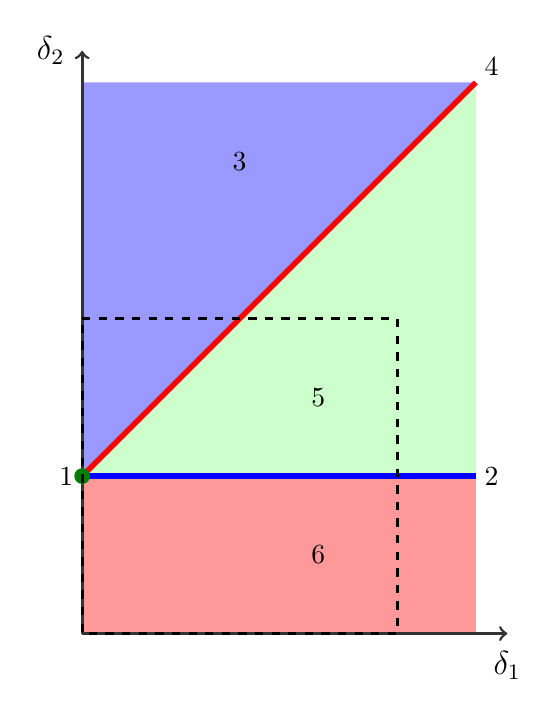
\begin{tikzpicture}[scale=.20]
	% STYLES
	\tikzstyle{axe} = [line width=1pt, ->, draw=black!80]
% 	\tikzstyle{goodzone} = [line width=2pt, draw=blue!50!black]
	\tikzstyle{v0} = [line width=1pt, draw=black, dashed]

	\tikzstyle{nomzone} = [draw=none, text=black]

	\tikzstyle{fondgris} = [fill=lightgray, draw=none]
	\tikzstyle{zone} = [draw=none]
	\tikzstyle{ligne} = [line width=2pt]

	% AXES
% 	\draw[fondgris] (0, 0) rectangle (3, 3);

	% ZONES
	% 3
	\draw[zone, fill=blue!40!white] (0, 35) -- (0, 10) -- (25, 35) -- cycle;
 	\node[nomzone] at (10, 30) {3};
	% 5
	\draw[zone, fill=green!20!white] (0, 10) -- (25, 35) -- (25, 10) -- cycle;
	\node[nomzone] at (15, 15) {5};
	% 6
	\draw[zone, fill=red!40!white] (0, 0) -- (0, 10) -- (25, 10) -- (25, 0) -- cycle;
	\node[nomzone] at (15, 5) {6};

	% AXES
	\path[axe]
		(0,0) -- ++ (27, 0);
	\path[axe]
		(0,0) -- ++ (0, 37);
	\node at (27, -2) {\large $\delta_1$};
	\node at (-2, 37) {\large $\delta_2$};
	
	% LINES
	% 4
	\draw[ligne, color=red] (0, 10) -- (25, 35);
 	\node[nomzone] at (26, 36) {4};
	% 2
	\draw[ligne, color=blue] (0, 10) -- (25, 10);
 	\node[nomzone] at (26, 10) {2};


	% POINT
	% 1
	\draw[zone, fill=green!50!black] (0,10) circle (.5);
 	\node[nomzone] at (-1, 10) {1};

	% GOOD ZONE
% 	\draw[goodzone]
% 		(8, 6) -- (8, 24) -- (9, 24) -- (27, 6) -- cycle;

	VO
	\path[v0]
		(0, 20) -- ++ (20, 0) -- ++ (0, -20) -- ++ (-20, 0) -- cycle;
	
	% VALEURS
% 	\foreach \x in {0, 1, ..., 40}
% 		\draw (0, \x) -- (-1, \x) node [left] {$\x$};
% 	\foreach \x in {0, 5, ..., 45}
% 		\draw (\x, 0) -- (\x, -1) node [below] {$\x$};
	
\end{tikzpicture}

\caption{Behavioral cartography of the SR latch according to $\delta_1$ and $\delta_2$}
\label{fig:sr_cartography}
\end{figure}
%-%-%-%-%-%-%-%-%-%-%-%-%-%-%-%-%-%-%-%-%-%-%-%-%%

Note that tile 1 corresponds to a point, and tiles 2 and 4 correspond to lines.

The rectangle $V_0$ has been represented with dashed lines.
% The number in (or next to) each tile represents the iteration number at which the corresponding constraint was computed during the algorithm run.
Note that all tiles (except tile~1) are unbounded, so that they cover, not only $V_0$, but all the positive real-valued plan.


The source code of this example is available in Appendix~\ref{app:source}.



%%%%%%%%%%%%%%%%%%%%%%%%%%%%%%%%%%%%%%%%%%%%%%%%%%%%%%%%%%%%%
%%%%%%%%%%%%%%%%%%%%%%%%%%%%%%%%%%%%%%%%%%%%%%%%%%%%%%%%%%%%%
\section*{Acknowledgments}
%%%%%%%%%%%%%%%%%%%%%%%%%%%%%%%%%%%%%%%%%%%%%%%%%%%%%%%%%%%%%
%%%%%%%%%%%%%%%%%%%%%%%%%%%%%%%%%%%%%%%%%%%%%%%%%%%%%%%%%%%%%

\'Etienne André instigated the development of \imitator{}, and keeps developing it.
Emmanuelle~Encrenaz and Laurent~Fribourg have been great contributors of \imitator{}, on a theoretical point of view, and to find applications both from the literature and real case studies.
Abdelrezzak~Bara provided several examples from the hardware literature.
Jeremy~Sproston provided examples from the probabilistic community.
Bertrand~Jeannet has been of great help on the linking with Apron~\cite{jm09} on a previous version of \imitator{}.
Ulrich~K\"uhne made several important improvements to \imitator{}, and linked the tool to PPL.
Daphne~Dussaud implemented the graphical output of the behavioral cartography.
Romain~Soulat implemented powerful algorithmic optimizations, and brought many case studies.

\imitator{}'s logo comes from KaterBegemot's \code{Typing monkey.svg} (Licence: Creative Commons Attribution-Share Alike 3.0 Unported).


%%%%%%%%%%%%%%%%%%%%%%%%%%%%%%%%%%%%%%%%%%%%%%%%%%%%%%%%%%%%%
%%%%%%%%%%%%%%%%%%%%%%%%%%%%%%%%%%%%%%%%%%%%%%%%%%%%%%%%%%%%%
\bibliographystyle{abbrv}
\bibliography{biblio}
%%%%%%%%%%%%%%%%%%%%%%%%%%%%%%%%%%%%%%%%%%%%%%%%%%%%%%%%%%%%%
%%%%%%%%%%%%%%%%%%%%%%%%%%%%%%%%%%%%%%%%%%%%%%%%%%%%%%%%%%%%%

\newpage

\appendix

%%%%%%%%%%%%%%%%%%%%%%%%%%%%%%%%%%%%%%%%%%%%%%%%%%%%%%%%%%%%%
%%%%%%%%%%%%%%%%%%%%%%%%%%%%%%%%%%%%%%%%%%%%%%%%%%%%%%%%%%%%%
\section{Source Code of the Example} \label{app:source}
%%%%%%%%%%%%%%%%%%%%%%%%%%%%%%%%%%%%%%%%%%%%%%%%%%%%%%%%%%%%%
%%%%%%%%%%%%%%%%%%%%%%%%%%%%%%%%%%%%%%%%%%%%%%%%%%%%%%%%%%%%%

%%%%%%%%%%%%%%%%%%%%%%%%%%%%%%%%%%%%%%%%%%%%%%%%%%%%%%%%%%%%%
\subsection{Main Input File}
%%%%%%%%%%%%%%%%%%%%%%%%%%%%%%%%%%%%%%%%%%%%%%%%%%%%%%%%%%%%%

\FichierImitator{include/SRlatch.imi}



%%%%%%%%%%%%%%%%%%%%%%%%%%%%%%%%%%%%%%%%%%%%%%%%%%%%%%%%%%%%%
\subsection{$V_0$ File}
%%%%%%%%%%%%%%%%%%%%%%%%%%%%%%%%%%%%%%%%%%%%%%%%%%%%%%%%%%%%%

\FichierImitator{include/SRlatch.v0}



\newpage

%%%%%%%%%%%%%%%%%%%%%%%%%%%%%%%%%%%%%%%%%%%%%%%%%%%%%%%%%%%%%
%%%%%%%%%%%%%%%%%%%%%%%%%%%%%%%%%%%%%%%%%%%%%%%%%%%%%%%%%%%%%
\section{Complete Grammar} \label{app:grammar}
%%%%%%%%%%%%%%%%%%%%%%%%%%%%%%%%%%%%%%%%%%%%%%%%%%%%%%%%%%%%%
%%%%%%%%%%%%%%%%%%%%%%%%%%%%%%%%%%%%%%%%%%%%%%%%%%%%%%%%%%%%%


%%%%%%%%%%%%%%%%%%%%%%%%%%%%%%%%%%%%%%%%%%%%%%%%%%%%%%%%%%%%%
\subsection{Grammar of the Input File}
%%%%%%%%%%%%%%%%%%%%%%%%%%%%%%%%%%%%%%%%%%%%%%%%%%%%%%%%%%%%%

\imitator{} input is described by the following grammar.
Non-terminals appear within angled parentheses.
A non-terminal followed by two colons is defined by the list of immediately following non-blank lines, each of which represents a legal expansion.
Input characters of terminals appear in typewritter font.
The meta symbol \emptystring{} denotes the empty string.

The text \npec{in green} is not taken into account by \imitator{}, but is allowed (or sometimes necessary) in order to allow the compatibility with \hytech{} files.


%------------------------------------------------------------
\regleGrammaire{imitator\_input}
%------------------------------------------------------------
\begin{tabular}{l l}
	\  & \nt{automata\_descriptions} \nt{init} \\
\end{tabular}

\medskip


We define each of those two components below.

%-%-%-%-%-%-%-%-%-%-%-%-%-%-%-%-%-%-%-%-%-%-%-%-%-%-%-%-%-%-%
\subsubsection{Automata Descriptions}
%-%-%-%-%-%-%-%-%-%-%-%-%-%-%-%-%-%-%-%-%-%-%-%-%-%-%-%-%-%-%

%------------------------------------------------------------
\regleGrammaire{automata\_descriptions}
%------------------------------------------------------------
\begin{tabular}{l l}
	\  & \nt{declarations} \nt{automata} \\
\end{tabular}

%------------------------------------------------------------
\regleGrammaire{declarations}
%------------------------------------------------------------
\begin{tabular}{l l}
	\  & \code{var} \nt{var\_lists} \\
\end{tabular}

%------------------------------------------------------------
\regleGrammaire{var\_lists}
%------------------------------------------------------------
\begin{tabular}{l l}
	\  & \nt{var\_list} \code{:} \nt{var\_type} \code{;} \nt{var\_lists} \\
	$|$ & \emptystring
\end{tabular}

%------------------------------------------------------------
\regleGrammaire{var\_list}
%------------------------------------------------------------
\begin{tabular}{l l}
	\  & \code{<name>} \\
	$|$ & \code{<name>} \code{,} \nt{var\_list}
\end{tabular}

%------------------------------------------------------------
\regleGrammaire{var\_type}
%------------------------------------------------------------
\begin{tabular}{l l}
	\  & \code{clock} \\
	$|$ & \code{discrete} \\
	$|$ & \code{parameter} \\
\end{tabular}

%------------------------------------------------------------
\regleGrammaire{automata}
%------------------------------------------------------------
\begin{tabular}{l l}
	\  & \nt{automaton} \nt{automata} \\
	$|$ & \emptystring \\
\end{tabular}

%------------------------------------------------------------
\regleGrammaire{automaton}
%------------------------------------------------------------
\begin{tabular}{l l}
	\  & \code{automaton} \code{<name>} \nt{prolog} \nt{locations} \code{end} \\
\end{tabular}

%------------------------------------------------------------
\regleGrammaire{prolog}
%------------------------------------------------------------
\begin{tabular}{l l}
	\  & \npec{\nt{initialization}} \nt{sync\_labels} \\
	$|$ & \nt{sync\_labels} \npec{\nt{initialization}} \\
	$|$ & \nt{sync\_labels} \\
\end{tabular}

%------------------------------------------------------------
\regleGrammaire{initialization}
%------------------------------------------------------------
\npec{
\begin{tabular}{l l}
	\  & \code{initially} \code{<name>} \nt{state\_initialization} \code{;} \\
\end{tabular}
}

%------------------------------------------------------------
\regleGrammaire{state\_initialization}
%------------------------------------------------------------
\npec{
\begin{tabular}{l l}
	\  & \code{\&} \nt{convex\_predicate} \\
	$|$ & \emptystring \\
\end{tabular}
}

%------------------------------------------------------------
\regleGrammaire{sync\_labels}
%------------------------------------------------------------
\begin{tabular}{l l}
	\  & \code{synclabs} \code{:} \nt{sync\_var\_list} \code{;} \\
\end{tabular}

%------------------------------------------------------------
\regleGrammaire{sync\_var\_list}
%------------------------------------------------------------
\begin{tabular}{l l}
	\  & \nt{sync\_var\_nonempty\_list} \\
	$|$ & \emptystring \\
\end{tabular}

%------------------------------------------------------------
\regleGrammaire{sync\_var\_nonempty\_list}
%------------------------------------------------------------
\begin{tabular}{l l}
	\  & \code{<name>} \code{,} \nt{sync\_var\_nonempty\_list} \\
	$|$ & \code{<name>} \\
\end{tabular}

%------------------------------------------------------------
\regleGrammaire{locations}
%------------------------------------------------------------
\begin{tabular}{l l}
	\  & \nt{location} \nt{locations} \\
	$|$ & \emptystring \\
\end{tabular}

%------------------------------------------------------------
\regleGrammaire{locations}
%------------------------------------------------------------
\begin{tabular}{l l}
	\  & \code{loc} \code{<name>} \code{:} \code{while} \nt{convex\_predicate} \nt{stop\_opt} \npec{\nt{wait\_opt}} \nt{transitions} \\
% 	$|$ & \code{loc} \code{<name>} \code{:} \code{while} \nt{convex\_predicate} \nt{transitions} \\
\end{tabular}

%------------------------------------------------------------
\regleGrammaire{wait\_opt}
%------------------------------------------------------------
\begin{tabular}{l l}
	\ & \npec{\code{wait()}} \\
	$|$ & \npec{\code{wait}} \\
	$|$ & \npec{\emptystring} \\
\end{tabular}

%------------------------------------------------------------
\regleGrammaire{stop\_opt}
%------------------------------------------------------------
\begin{tabular}{l l}
	\ & \code{stop\{} \nt{var\_list} \code{\}} \\
	$|$ & \emptystring \\
\end{tabular}

	
%------------------------------------------------------------
\regleGrammaire{transitions}
%------------------------------------------------------------
\begin{tabular}{l l}
	\  & \nt{transition} \nt{transitions} \\
	$|$ & \emptystring \\
\end{tabular}

%------------------------------------------------------------
\regleGrammaire{transition}
%------------------------------------------------------------
\begin{tabular}{l l}
	\  & \code{when} \nt{convex\_predicate} \nt{update\_synchronization} \code{goto} \code{<name>} \code{;} \\
\end{tabular}

%------------------------------------------------------------
\regleGrammaire{update\_synchronization}
%------------------------------------------------------------
\begin{tabular}{l l}
	\  & \nt{updates} \\
	$|$ & \nt{syn\_label} \\
	$|$ & \nt{updates} \nt{syn\_label} \\
	$|$ & \nt{syn\_label} \nt{updates} \\
	$|$ & \emptystring \\
\end{tabular}

%------------------------------------------------------------
\regleGrammaire{updates}
%------------------------------------------------------------
\begin{tabular}{l l}
	\  & \code{do} \code{(} \nt{update\_list} \code{)} \\
\end{tabular}

%------------------------------------------------------------
\regleGrammaire{update\_list}
%------------------------------------------------------------
\begin{tabular}{l l}
	\  & \nt{update\_nonempty\_list} \\
	$|$ & \emptystring \\
\end{tabular}

%------------------------------------------------------------
\regleGrammaire{update\_nonempty\_list}
%------------------------------------------------------------
\begin{tabular}{l l}
	\  & \nt{update} \code{,} \nt{update\_nonempty\_list} \\
	$|$ & \nt{update} \\
\end{tabular}

%------------------------------------------------------------
\regleGrammaire{update}
%------------------------------------------------------------
\begin{tabular}{l l}
	\  & \code{<name>} \code{'} \code{=} \nt{linear\_expression} \\
\end{tabular}

%------------------------------------------------------------
\regleGrammaire{syn\_label}
%------------------------------------------------------------
\begin{tabular}{l l}
	\  & \code{sync} \code{<name>} \\
\end{tabular}



%------------------------------------------------------------
\regleGrammaire{convex\_predicate}
%------------------------------------------------------------
\begin{tabular}{l l}
	\  & \nt{linear\_constraint} \code{\&} \nt{convex\_predicate} \\
	$|$ & \nt{linear\_constraint} \\
\end{tabular}

%------------------------------------------------------------
\regleGrammaire{linear\_constraint}
%------------------------------------------------------------
\begin{tabular}{l l}
	\  & \nt{linear\_expression} \nt{relop} \nt{linear\_expression} \\
	$|$ & \code{True} \\
	$|$ & \code{False} \\
\end{tabular}

%------------------------------------------------------------
\regleGrammaire{relop}
%------------------------------------------------------------
\begin{tabular}{l l}
	\  & \code{<} \\
	$|$ & \code{<=} \\
	$|$ & \code{=} \\
	$|$ & \code{>=} \\
	$|$ & \code{>} \\
\end{tabular}

%------------------------------------------------------------
\regleGrammaire{linear\_expression}
%------------------------------------------------------------
\begin{tabular}{l l}
	\  & \nt{linear\_term} \\
	$|$ & \nt{linear\_expression} \code{+} \nt{linear\_term} \\
	$|$ & \nt{linear\_expression} \code{-} \nt{linear\_term} \\
\end{tabular}

%------------------------------------------------------------
\regleGrammaire{linear\_term}
%------------------------------------------------------------
\begin{tabular}{l l}
	\  & \nt{rational} \\
	$|$ & \nt{rational} \code{<name>} \\
	$|$ & \nt{rational} \code{*} \code{<name>} \\
	$|$ & \code{<name>} \\
	$|$ & \code{(} \nt{linear\_term} \code{)} \\
\end{tabular}

%------------------------------------------------------------
\regleGrammaire{rational}
%------------------------------------------------------------
\begin{tabular}{l l}
	\  & \nt{integer} \\
	\  & \nt{float} \\
	$|$ & \nt{integer} \code{/} \nt{pos\_integer}  \\
\end{tabular}

%------------------------------------------------------------
\regleGrammaire{integer}
%------------------------------------------------------------
\begin{tabular}{l l}
	\  & \nt{pos\_integer} \\
	$|$ & \code{-} \nt{pos\_integer}  \\
\end{tabular}

%------------------------------------------------------------
\regleGrammaire{pos\_integer}
%------------------------------------------------------------
\begin{tabular}{l l}
	\  & \code{<int>} \\
\end{tabular}



%------------------------------------------------------------
\regleGrammaire{float}
%------------------------------------------------------------
\begin{tabular}{l l}
	\  & \nt{pos\_float} \\
	$|$ & \code{-} \nt{pos\_float}  \\
\end{tabular}


%------------------------------------------------------------
\regleGrammaire{pos\_float}
%------------------------------------------------------------
\begin{tabular}{l l}
	\  & \code{<float>} \\
\end{tabular}


%-%-%-%-%-%-%-%-%-%-%-%-%-%-%-%-%-%-%-%-%-%-%-%-%-%-%-%-%-%-%
\subsubsection{Initial State}
%-%-%-%-%-%-%-%-%-%-%-%-%-%-%-%-%-%-%-%-%-%-%-%-%-%-%-%-%-%-%

%------------------------------------------------------------
\regleGrammaire{init}
%------------------------------------------------------------
\begin{tabular}{l l}
	& \npec{\nt{init\_declaration}} \nt{init\_definition} \nt{bad\_definition} \npec{\nt{reach\_command}} \\
	$|$  & \npec{\nt{init\_declaration}} \nt{init\_definition} \npec{\nt{reach\_command}} \\
\end{tabular}

%------------------------------------------------------------
\regleGrammaire{init\_declaration}
%------------------------------------------------------------
\begin{tabular}{l l}
	\  & \npec{\code{var} \code{init} \code{:} \code{region} \code{;}} \\
	$|$ & \emptystring \\
\end{tabular}

%------------------------------------------------------------
\regleGrammaire{reach\_command}
%------------------------------------------------------------
\begin{tabular}{l l}
	\  & \npec{\code{print} \code{(} \code{reach} \code{forward} \code{from} \code{init} \code{endreach} \code{)} \code{;}} \\
	$|$ & \emptystring \\
\end{tabular}

%------------------------------------------------------------
\regleGrammaire{init\_definition}
%------------------------------------------------------------
\begin{tabular}{l l}
	\  & \code{init} \code{:=} \nt{region\_expression} \code{;} \\
\end{tabular}

%------------------------------------------------------------
\regleGrammaire{region\_expression}
%------------------------------------------------------------
\begin{tabular}{l l}
	\  & \nt{state\_predicate} \\
	$|$ & \code{(} \nt{region\_expression} \code{)} \\
	$|$ & \nt{region\_expression} \code{\&} \nt{region\_expression} \\
\end{tabular}

%------------------------------------------------------------
\regleGrammaire{state\_predicate}
%------------------------------------------------------------
\begin{tabular}{l l}
	\  & \code{loc} \code{[} \code{<name>} \code{]} \code{=} \code{<name>} \\
	$|$ & \nt{linear\_constraint} \\
\end{tabular}

%------------------------------------------------------------
\regleGrammaire{bad\_definition}
%------------------------------------------------------------
\begin{tabular}{l l}
	\  & \code{bad := } \nt{loc\_expression} \code{;} \\
\end{tabular}

%------------------------------------------------------------
\regleGrammaire{loc\_expression}
%------------------------------------------------------------
\begin{tabular}{l l}
	\  & \nt{loc\_predicate} \\
	$|$ & \nt{loc\_predicate} \code{\&} \nt{loc\_expression} \\
	$|$ & \nt{loc\_predicate} \nt{loc\_expression} \\
\end{tabular}

%------------------------------------------------------------
\regleGrammaire{loc\_predicate}
%------------------------------------------------------------
\begin{tabular}{l l}
	\  & \code{loc[} \code{<name>} \code{] = \code{<name>}} \\
\end{tabular}


%%%%%%%%%%%%%%%%%%%%%%%%%%%%%%%%%%%%%%%%%%%%%%%%%%%%%%%%%%%%%
% \subsection{Grammar of reference valuation file}
%%%%%%%%%%%%%%%%%%%%%%%%%%%%%%%%%%%%%%%%%%%%%%%%%%%%%%%%%%%%%
% TO DO 

%%%%%%%%%%%%%%%%%%%%%%%%%%%%%%%%%%%%%%%%%%%%%%%%%%%%%%%%%%%%%
% \subsection{Grammar of reference rectangle file}
%%%%%%%%%%%%%%%%%%%%%%%%%%%%%%%%%%%%%%%%%%%%%%%%%%%%%%%%%%%%%
% TO DO 


%%%%%%%%%%%%%%%%%%%%%%%%%%%%%%%%%%%%%%%%%%%%%%%%%%%%%%%%%%%%%
\subsection{Reserved Words}
%%%%%%%%%%%%%%%%%%%%%%%%%%%%%%%%%%%%%%%%%%%%%%%%%%%%%%%%%%%%%

The following words are keywords and cannot be used as names for automata, variables, synchronization labels or locations. 

\code{and},
\code{automaton},
\code{bad},
\code{clock},
\code{discrete},
\code{do},
\code{end},
% \code{endreach},
\code{False},
% \code{forward},
% \code{from},
\code{goto},
\code{if},
% \code{in},
\code{init},
\code{initially},
\code{loc},
\code{locations},
\code{not},
\code{or},
\code{parameter},
% \code{print},
% \code{reach},
\code{region},
\code{sync},
\code{stop},
\code{synclabs},
\code{True},
\code{var},
\code{wait},
\code{when},
\code{while}

\end{document}

